\subsection{An\'alise Explorat\'oria dos Dados}

Os dados foram processados usando a EDA  \cite{Bandara2021} resumindo suas principais características, e formulando hipóteses que possam direcionar a coleta adicional de dados, se necessária. 

Existem dados anômalos \textit{Not a Number} (NAN) que representam a ausência de dados coletados, logo tais dados foram interpolados usando os valores existentes e vizinhos a ele. 

Assim como em qualquer empresa de saneamento básico e tratamento de água, é utilizado um mecanismo de acionamento automático denominado trava de segurança para evitar que o nível do tanque se aproxime de zero e haja falta de água nos locais abastecidos por esse tanque. O nível máximo que o tanque pode alcançar é de $5,26 m^3$ (equivalente a $5264.56$ litros). As bombas são ativadas em sua potência máxima para evitar que sejam acionadas quando o nível do tanque estiver dentro dessa faixa. No entanto, a bomba $1$ ainda estaria operando para completar o nível do tanque caso esteja dentro dessa faixa. 

Na Tabela \ref{tb:est}, o desvio padrão é representado por \textit{STandard Deviation} (STD). A quantidade de dados medidos hora a hora pela SANEPAR de $2018$ a $2019$ são de $17.522$ dados.

\begin{table}[!htb]
	\centering
	\caption{Descrição estatística dos dados do Bairro Alto em Curitiba de 2018 a 2019 disponibilizados pela SANEPAR.}\label{tb:est}
	\begin{tabular}{@{}llllllllll@{}}
		\toprule
		\text{Métricas} & \text{B1} & \text{B2} & \text{B3} & \text{LT01} & \text{FT01} & \text{FT02} & \text{FT03} & \text{PT01} & \text{PT02} \\ \midrule
		\textbf{Média}    & 52,289      & 18,421      & 3,338       & 3,513         & 215,699       & 114,832       & 104,195       & 4,448         & 20,724        \\
		\textbf{STD}      & 11,421      & 19,742      & 12,624      & 0,670         & 110,223       & 43,604        & 25,636        & 0,700         & 3,610         \\
		\textbf{Min.}     & 0           & 0           & 0           & 0,294         & 0             & 0             & 0             & 0,842         & 0             \\
		\textbf{25\%}     & 49,519      & 0           & 0           & 3,077         & 255,454       & 74,912        & 81,430        & 4,015         & 18,072        \\
		\textbf{50\%}     & 57,925      & 0,050       & 0           & 3,715         & 265,357       & 122,149       & 109,911       & 4,602         & 21,791        \\
		\textbf{75\%}     & 57,989      & 36,796      & 0           & 4,047         & 272,609       & 145,865       & 123,189       & 4,990         & 23,051        \\
		\textbf{Max.}     & 59,988      & 59,992      & 59,988      & 4,445         & 390,683       & 400,415       & 183,900       & 5,639         & 29,008        \\ \bottomrule
	\end{tabular}
\end{table}

No contexto de análises de dados várias técnicas de EDA têm sido adotadas.
Neste estudo serão abordadas várias análises entre elas correlação de Pearson, para verificar quais variáveis podem ser excluídas tais como ruídos (correlação baixa) ou altamente correlacionadas com a variável de saída do nosso estudo, que será a variável LT01, nível do tanque de armazenamento de água pela SANEPAR no Bairro Alto. Nesse caso, as variáveis removidas tem pouca correlação com a LT01, as que apresentam correlação baixa são B3 e FT02 e serão removidas.

A Figura \ref{fig:person} mostra a correlação de Pearson entre as variáveis do conjunto de dados deste estudo. Essa figura representa a matriz (simétrica) da dependência/correlação entre as variáveis. Analisamos as correlações das variáveis de entrada com a variável de saída. Serão descartadas as variáveis com correlação menor que 5\% e maior que 90\%.

\begin{figure}[!htb]
	\centering
	\caption{Correlação de Pearson.}
	\label{fig:person}	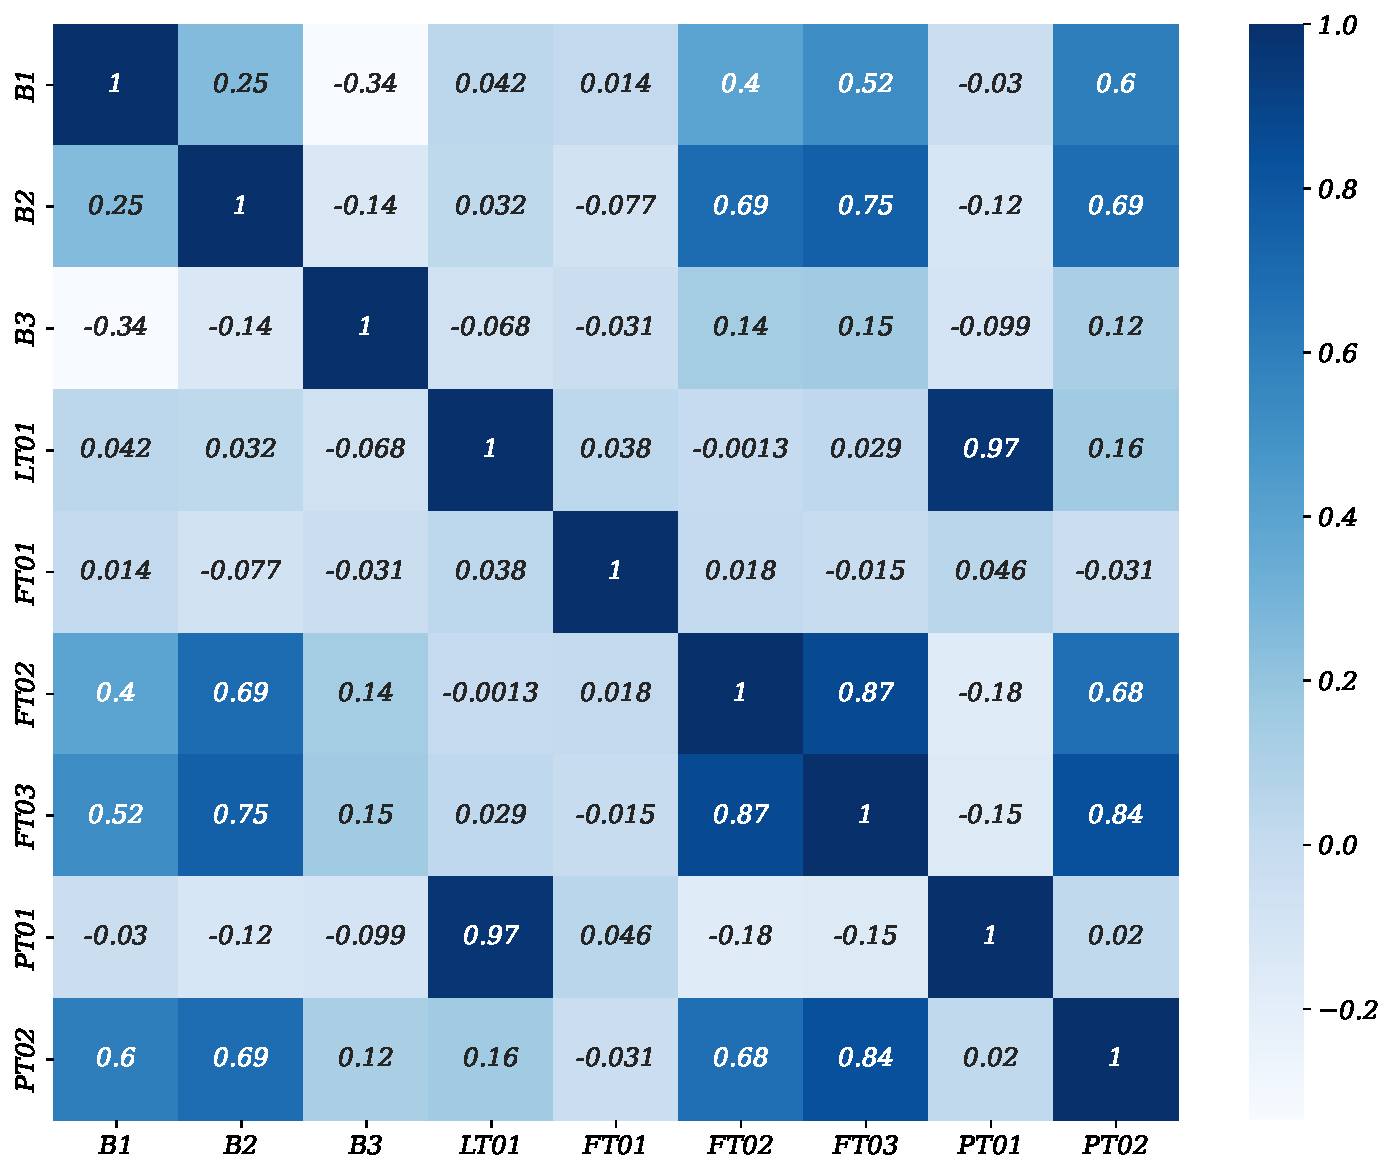
\includegraphics[width=0.7\linewidth]{Resultados/Figuras/person}
		
\end{figure}

Nesse conjunto de dados que está sendo trabalhado, há uma forte correlação da variável PT01 com o LT01 conforme visto na Figura \ref{fig:lr-lt01-m3} que fornece uma representação dos coeficientes $\beta_0$ e $\beta_1$, que são os coeficientes da correlação linear entre as variáveis. Um aumento de $1$ na variável $x$ está associado a um aumento proporcional de $\beta_1$ na variável $y$. O valor de $\beta_0$ representa o valor de $y$ quando $x$ é igual a $0$.

\begin{figure}[!htb]
	\centering
	\caption{Relação entre LT01 e PT01 cuja correlação de Pearson é 97\%}
	\label{fig:lr-lt01-m3}
	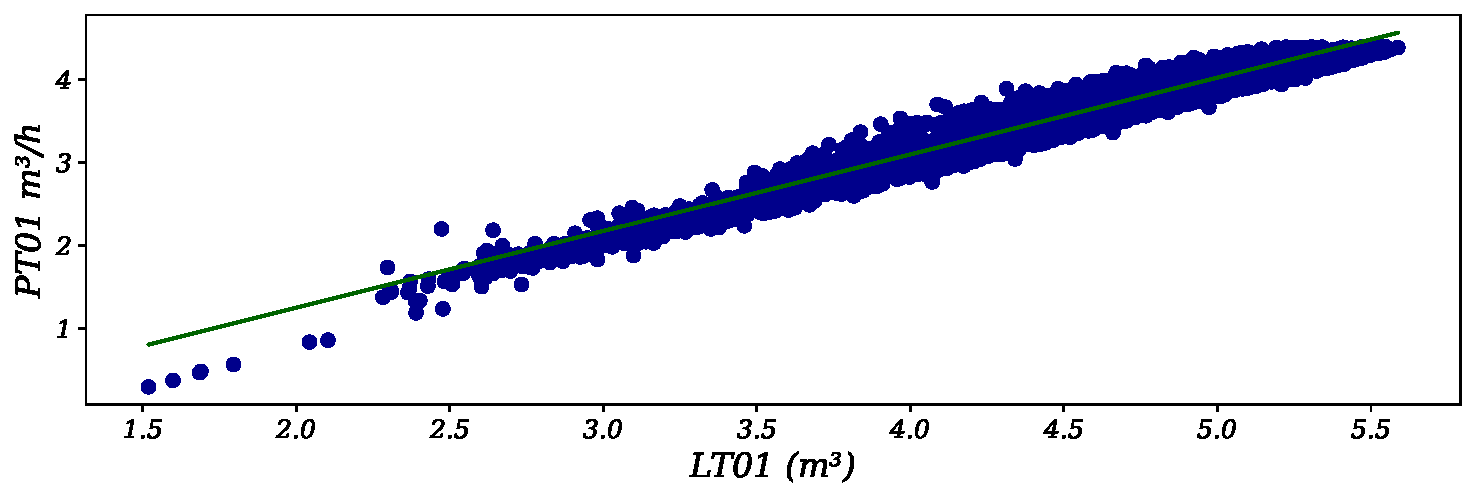
\includegraphics[width=0.7\linewidth]{Resultados/Figuras/LR}
\end{figure}

\textit{Augmented Dickey-Fuller} (ADF) de $-12,515$ indica a evidência de estacionariedade na série temporal. 
O valor de p expresso como $2,62\times 10^{-23}$ está associado ao teste ADF. Este valor-p representa a probabilidade de obter um resultado igual ou mais extremo do que o observado, sob a suposição de que a hipótese nula seja verdadeira. No contexto do teste ADF, a hipótese nula é a presença de raiz unitária na série temporal, indicando não estacionariedade. Dado o valor de p de $2,62\times 10^{-23}$, evidencia-se uma probabilidade muito baixa, indicando forte suporte contra a hipótese nula e sugerindo que a série temporal é estacionária. Na Tabela \ref{tb:adf}, são apresentados todos os dados do teste para estacionariedade.Os resultados indicam fortes evidências contra a hipótese nula. Com um teste ADF de $-12,515 $ e um valor de p extremamente baixo de $2,62 \times 10^{-23}$, rejeita-se a hipótese nula de presença de raiz unitária. Os $44$ atrasos utilizados e as $17.477$ observações corroboram a análise estatística. Ao comparar a estatística de teste ADF com os valores críticos, observa-se que está significativamente abaixo deles em todos os níveis de significância $(1\%, 5\%, 10\%)$. Portanto, a conclusão é de que os dados não possuem raiz unitária, indicando que são estacionários.

\begin{table}[!htb]
	\centering
	\caption{Teste ADF.}\label{tb:adf}
	\begin{tabular}{ll}
		\hline
		Valor de p & $2,62 \times 10^{-23}$ \\
		Atrasos utilizados & $44$ \\
		Número de observações & $17.477$ \\
		Valor crítico $(1\%)$ & $-3,431$ \\
		Valor crítico $(5\%)$ & $-2,862$ \\
		Valor crítico $(10\%)$ & $-2,567$ \\
		\hline
	\end{tabular}
\end{table}


As figuras contendo os gráficos ACF e PACF são ferramentas essenciais na análise de séries temporais, especialmente ao trabalhar com modelos ARIMA. 

O ACF é uma medida estatística utilizada para identificar a presença de correlação serial em uma série temporal. Ele calcula a autocorrelação entre os valores da série em diferentes defasagens, ou seja, a correlação entre os valores atuais e os valores passados da série. O ACF é útil para analisar a dependência temporal dos dados e identificar padrões de sazonalidade, tendência ou outros efeitos temporais. Por meio do ACF, é possível avaliar se a série exibe autocorrelação significativa em defasagens específicas, o que pode indicar a presença de não estacionariedade ou estrutura temporal que precisa ser considerada na análise ou modelagem da série temporal.

Enquanto o ACF mede a correlação total em um determinado lag, o PACF mede a correlação apenas entre a observação atual e uma observação em um lag específico, controlando os efeitos das observações intermediárias. O gráfico PACF é especialmente útil para identificar a ordem do componente autorregressivo (AR) no modelo ARIMA. Ele ajuda a identificar os lags que têm uma influência direta na observação atual, sem a interferência de outros lags. Ao usar esses gráficos em conjunto, os analistas de séries temporais podem identificar a ordem adequada do modelo ARIMA. 

A ordem do ARIMA é denotada como ($p, d, q$), onde p é a ordem do componente AR, d é a ordem de diferenciação, que representa o número de vezes que a série temporal é diferenciada para torná-la estacionária, e q é a ordem do componente de MA. Os pontos nos gráficos ACF e PACF que ultrapassam as bandas de confiança indicam lags significativos. Analisando esses gráficos, pode fazer escolhas sobre os valores de $p$, $d$, e $q$ ao ajustar um modelo ARIMA à série temporal em questão. 

Na Figura \ref{fig:acfa}, pode-se observar a diferença entre ACF exibida na Figura \ref{fig:acfa} e PACF exibida na Figura \ref{fig:pacf}. A autocorrelação é uma medida da correlação entre os valores da série temporal em diferentes defasagens, levando em consideração tanto a correlação direta quanto a correlação indireta. Por outro lado, a autocorrelação parcial mede apenas a correlação direta entre os valores, desconsiderando a influência das defasagens intermediárias. Essas análises são úteis para identificar padrões e relações de dependência entre os valores da série temporal, fornecendo informações importantes para a modelagem e previsão desses dados. O intervalo de confiança padrão de $95\%$ é representado pela faixa azul nas Figuras \ref{fig:acfa} e \ref{fig:pacf}. As observações que estão fora desse intervalo são consideradas estatisticamente correlacionadas, indicando a presença de padrões ou estrutura na série temporal.

A correlação visualizada na Figura \ref{fig:acfa} é fundamental para a interpretação do teste ADF. Em uma série de ruído branco, os valores são completamente aleatórios e não apresentam correlação significativa. Portanto, quando há correlação presente na série, isso indica a existência de padrões ou dependências entre os valores, o que pode ser explorado para a modelagem e previsão da série temporal.

\begin{figure}[!htb]
	\centering
\caption{Autocorrelação.}\label{fig:acfa}	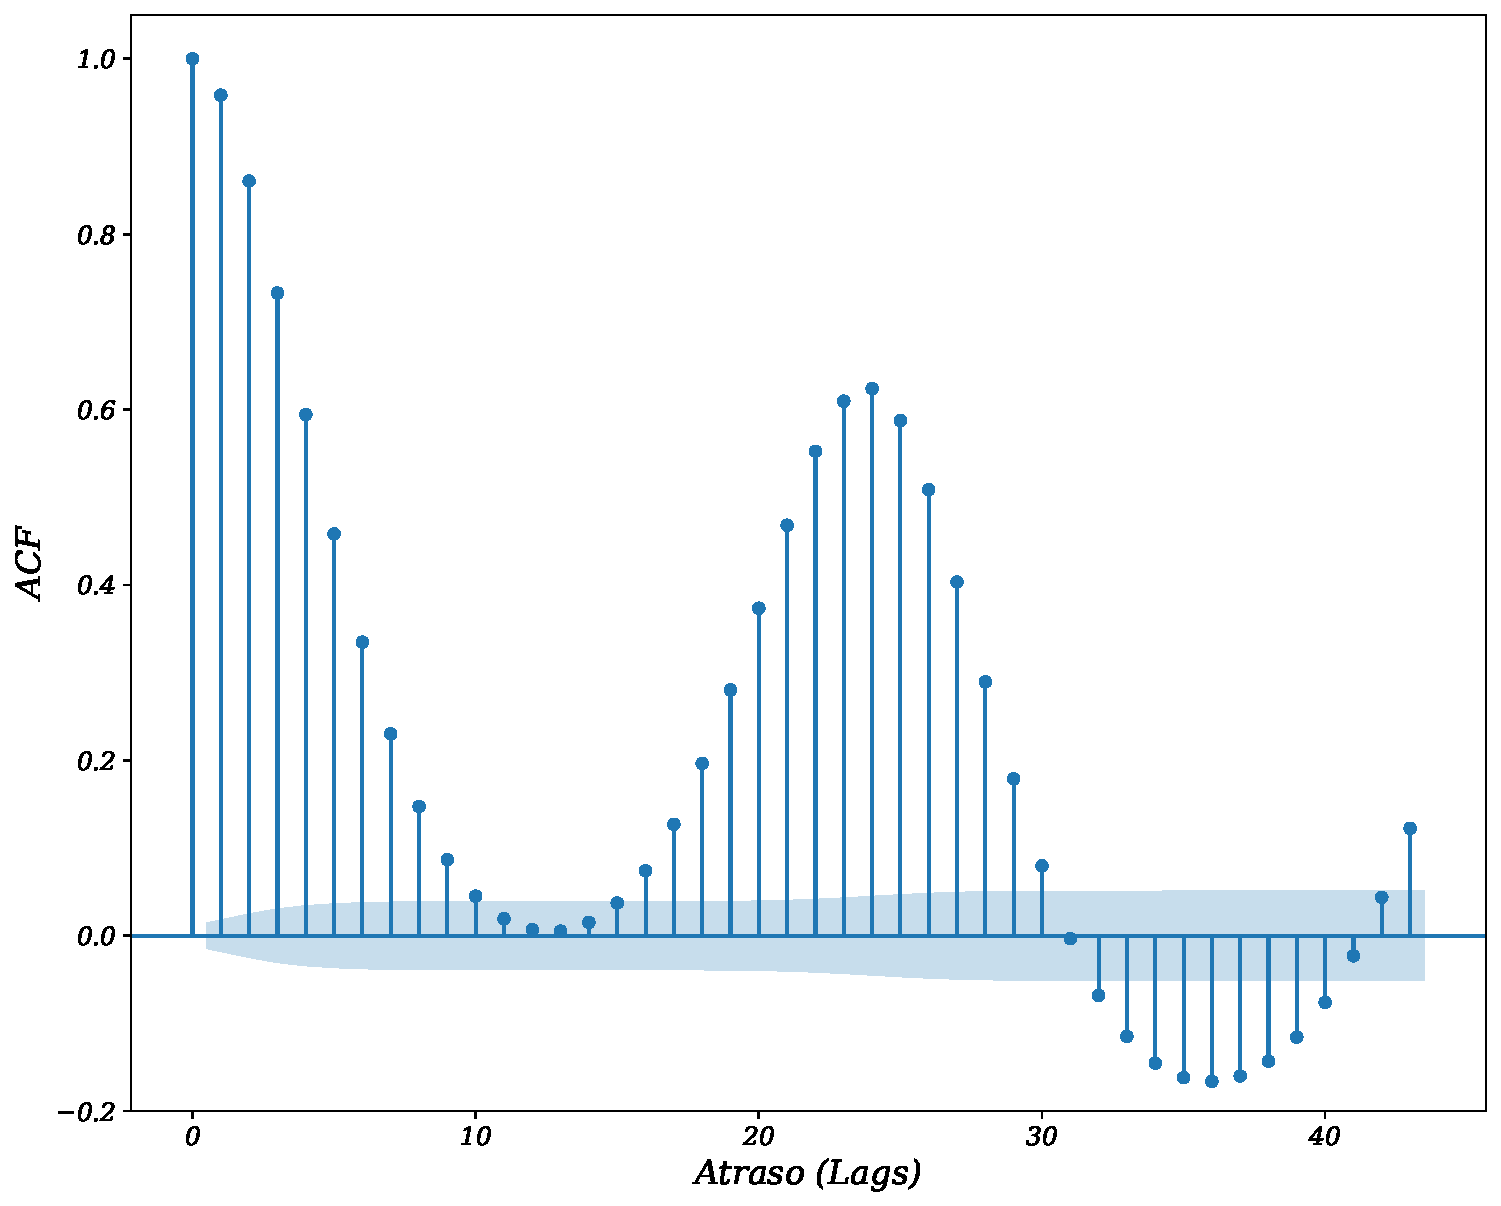
\includegraphics[width=0.7\linewidth]{Resultados/Figuras/acf} 
\end{figure}

\begin{figure}[!htb]
	\centering
	\caption{Autocorrelação parcial.}\label{fig:pacf}	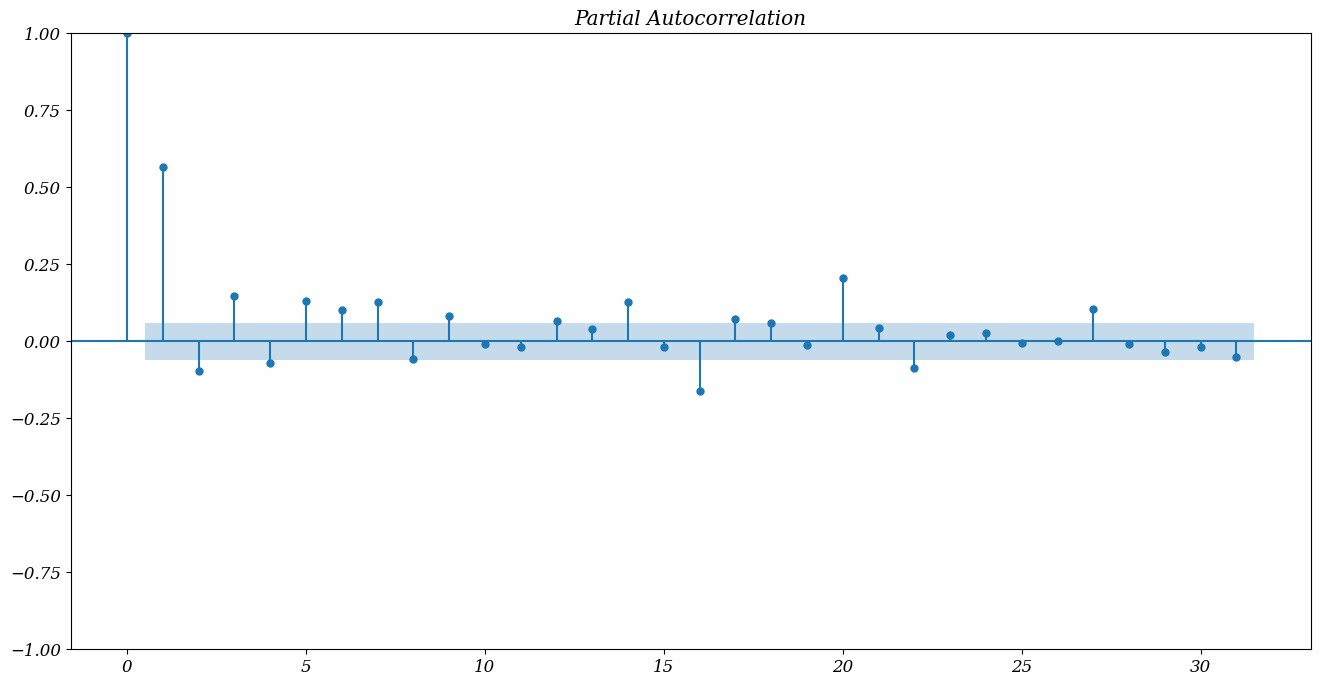
\includegraphics[width=0.7\linewidth]{Resultados/Figuras/pacf}
\end{figure}

Demonstrar que uma série temporal tem ou pode ter um ruído branco também é conveniente para a análise da EDA.
Na Figura \ref{fig:ruido-branco}, é possível observar uma série temporal que pode ser caracterizada como ruído branco, se suas variáveis forem independentes e distribuídas de forma idêntica, com média zero. Isso implica que todas as variáveis possuem a mesma variância ($\sigma^2$) e que cada valor não possui correlação com os demais valores da série.

\begin{figure}[!htb]
	\centering
	\caption{Ruído branco.}
	\label{fig:ruido-branco}
	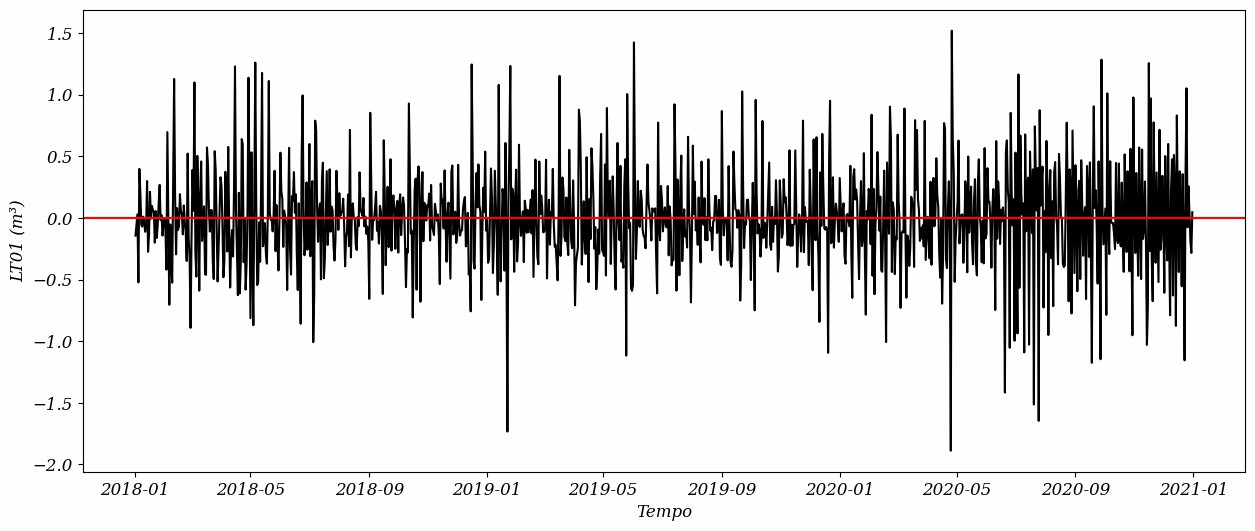
\includegraphics[width=\linewidth]{Resultados/Figuras/ruido-branco}
\end{figure}

Com a decomposição STL é possível analisar se a série apresenta tendência, sazonalidade e ruídos. Ao observar a Figura \ref{fig:stl}, é evidente que os dados exibem ambos os padrões. 

\begin{figure}[!htb]
	\centering
	\caption{Decomposição STL aditiva.}
	\label{fig:stl}
	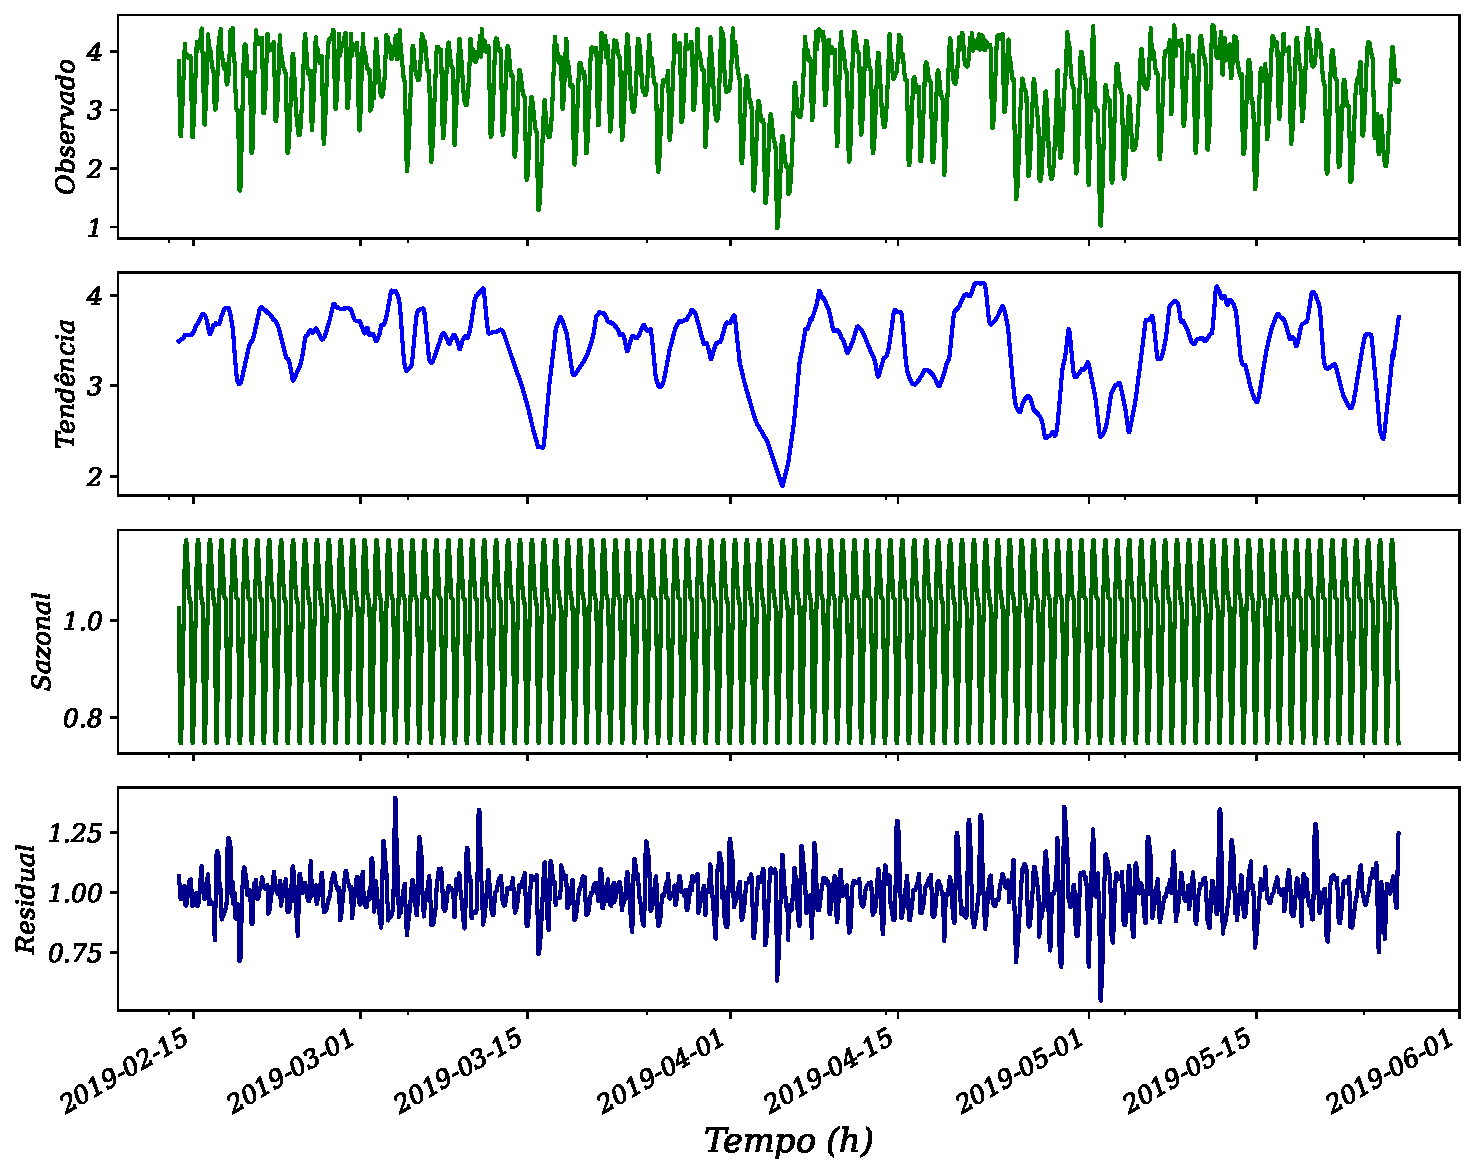
\includegraphics[width=\linewidth]{Resultados/Figuras/STL}	
\end{figure}


Essa decomposição divide os dados em sazonalidade, para descobrir no modelo ARIMA e seus antecessores que os dados podem ser coletados por hora, dia, mês ou ano. Saber que uma série tem sazonalidade torna o modelo ARIMA mais robusto, permitindo o uso do modelo ARIMA com sazonalidade, conhecido como SARIMA. Esses dados, por representarem uma sazonalidade difícil de ser notada, resultam em modelos com essa sazonalidade que não apresentam muita redução nos valores dos erros.

A tendência dos dados reflete como a série se comporta ao longo prazo, se ela pode subir ou reduzir o padrão. Tanto uma série pode ser estacionária ou não estacionária. Pela Figura \ref{fig:stl}, a tendência parece ser linear, caracterizando a série como estacionária. No entanto, essa série não possui um padrão sazonal, o que faz com que os modelos de ARIMA com sazonalidade apresentem erros maiores em comparação aos modelos clássicos.

O resíduo nos dados da série temporal é uma forma de avaliar que a série trabalhada possui várias irregularidades, levando aos resíduos que ajudam a verificar a verdadeira essência dos dados. Como esses dados foi coletado por hora ele tem muita oscilação, trazendo muitos ruídos ao longo da análise.


Para a previsão os dados foram divididos em conjuntos de treinamento, validação, e teste \cite{raschka2015practical, geron2017hands_on}. Quanto à divisão dos dados, foi adotada uma estratégia básica em que $70\%$ dos dados foram destinados ao conjunto de treinamento e $30\%$ restantes foram reservados para o conjunto de teste. Dentro dos $70\%$ de treinamento, foi realizada uma subdivisão em que $80\%$ desses dados foram usados novamente para treinamento e os $20\%$ restantes foram utilizados para validação. 

A estratégia recursiva é mencionada por \citeonline{PETROPOULOS2022705} como uma abordagem eficaz na previsão de séries temporais de múltiplos passos. De acordo com o autor, essa estratégia envolve o uso de previsões anteriores como entradas para prever os próximos passos da série temporal. A abordagem recursiva tem demonstrado potencial para melhorar a acurácia das previsões de séries temporais de longo prazo.

MISO foi o modelo usado neste estudo. O modelo ARIMA, juntamente com suas variantes e extensões, foi amplamente estudado durante a pesquisa, assim como modelos regressivos que envolvem múltiplas variáveis de entrada e uma variável de saída, neste caso, a LT01. As demais variáveis foram utilizadas como suporte para melhorar o modelo do tipo ARIMAX, modelos com variáveis exógenas. 

Quando aplicado sem o uso de variáveis exógenas, o modelo ARIMA apresenta apenas uma entrada, semelhante ao modelo de \textit{Linear Regression}. No entanto, ao incluir variáveis exógenas, o modelo se torna MISO, permitindo uma modelagem  abrangente e considerando a correlação das várias para prever a variável de interesse, LT01.

A previsão dos dados foi feita com diferentes horizontes de previsão como $1$ hora, $6$ horas, $12$ horas, e $24$ horas. Essas estratégias de previsão permitem a comparação entre os modelos de regressão e modelos ARIMA em diferentes horizontes temporais.

Além desses modelos de previsão, vários outros modelos foram utilizados no estudo, tais como DT, RF, XGBoost, LightGBM, MLP, LSTM, GRU, Prophet, RNN, e CNN, a fim de obter o melhor resultado para a previsão de séries temporais de abastecimento de água.

Foram utilizados os parâmetros obtidos pelo autoARIMA que são $(p = 7, d = 0, q = 0) (P = 2, D = 1, Q = 1)_{M = 12}$, que foram ajustados para obter um melhor resultado, sendo $(p = 7, d = 1, q = 7) (P = 2, D = 1, Q = 1)_{M = 12}$. 

Na Tabela \ref{tab:autoarima_params} são exibidos todos os valores obtidos pela função autoARIMA e ajustados para que obtenham o melhor resultado para $p$ que é a ordem do componente AR, $d$ que é o número de diferenciações não sazonais, $q$ que é a ordem do componente MA, $P$ que é a ordem do componente AR sazonal, $D$ que é o número de diferenciações sazonais, $Q$ que é a ordem do componente MA sazonal, $M$ que é o período sazonal (número de observações em um ciclo sazonal).

\begin{table}[!htb]
	\centering
	\caption{Parâmetros para os modelos ARIMA utilizando a função autoARIMA.}
	\label{tab:autoarima_params}
	\small
	\begin{tabular}{ll}
	\toprule
	\text{Modelos} & \text{Parâmetros}   \\
	\midrule
		AR(p) & \( p = 7 \)  \\
		ARX(p) & \( p = 7 \) \\
		MA(q) & \( q = 7 \)   \\
		ARMA(p, q) & \( p = 7 \), \( q = 7 \)  \\
		ARIMA(p, d, q) & \( p = 7 \), \( d = 1 \), \( q = 7 \)  \\
		ARIMAX(p, d, q) & \( p = 7 \), \( d = 1 \), \( q = 7 \)  \\
		SARIMA(p, d, q)(P, D, Q) & \( p = 7 \), \( d = 1 \), \( q = 7 \), \( P = 2 \), \( D = 1 \), \( Q = 1 \) \\
		SARIMAX(p, d, q)(P, D, Q, M) & \( p = 7 \), \( d = 1 \), \( q = 7 \), \( P = 2 \), \( D = 1 \), \( Q = 1 \), \( M = 12 \)\\
		\bottomrule
	\end{tabular}
\end{table}

Os hiperparâmetros dos modelos foram otimizados usando a biblioteca Optuna do Python. Nesse contexto, foram empregadas técnicas bayesianas, especificamente o algoritmo TPE visando uma otimização mais eficiente.

Na Tabela \ref{tab:hiperparametros} são descritos os hiperparâmetros dos modelos XGBoost, LightGBM, RF, e DT, onde NE é o número de estimadores, PM é a profundidade máxima, MAD é o mínimo de amostras por divisão, MAF é o mínimo de amostras por folha, e TA é a taxa de aprendizado. 

\begin{table}[!htb]
	\centering
	\caption{Hiperparâmetros otimizados dos modelos.}
	\label{tab:hiperparametros}
	\begin{tabular}{llllll}
		\toprule
		\text{Modelo} & \text{Estimadores} & \text{PM} & \text{MAD} & \text{MAF} & \text{TA} \\
		\midrule
		XGBoost & 503 & 5 & 7 & 2  & 0,034 \\
		LightGBM & 820 & 10 & 3 & 5 & 0,014 \\
		RF & 135 & 10 & 4 & 2 & N/A \\
		DT & N/A & 229 & 32 & 20 & N/A \\
		\bottomrule
	\end{tabular}
\end{table}

Os hiperparâmetros dos modelos de rede neural artificial, como RNN, MLP, CNN, GRU, e LSTM obtidos pela otimização do Optuna são exibidos na Tabela \ref{tab:hyperparameters_summary}. CNN usou kernel 7 e densas 1, enquanto MLP usou densas 1.

\begin{table}[!htb]
	\centering
	\caption{Hiperparâmetros otimizados para RNA.}
	\label{tab:hyperparameters_summary}
	\small
	\begin{tabular}{lllll}
		\toprule
		\text{Modelo} & \text{Layers} & \text{Tamanho} & \text{No. Épocas} & \text{Dropout/} \\
		&&\text{do Batch}&& \text{Learning Rate}\\
		\midrule
		LSTM & 128 & 32 & 77 & -- \\
		GRU & -- & 32 & 50 & --  \\
		RNN & 79 & 16 & 50 & 0,0008612 \\
		CNN & -- & 61 & 10 & 0,2799; 0,00052 \\
		MLP & 125 & 27 & 96 & 0,4135, 0,0004057 \\
		\bottomrule
	\end{tabular}
\end{table}

\subsection{Aplicando os Modelos de Previs\~ao}

Foram empregadas três métricas estatísticas para avaliar e comparar o desempenho dos modelos de previsão.

Na análise dos modelos desenvolvidos, observou-se que o modelo RNN obteve o melhor desempenho, tanto para previsões de curto prazo, durante as horas de pico entre 18h e 21h, quanto para outros períodos. Além disso, os modelos MA, AR, SARIMA, ARIMA, SARIMAX, ARIMAX, ARX, LightGBM, XGBoost, RF, RNN, MLP, CNN, GRU, LSTM, e Prophet também apresentaram resultados satisfatórios, seguindo uma ordem decrescente de desempenho.

Uma observação recorrente foi a superioridade dos modelos que incorporam variáveis exógenas em termos de capacidade de previsão, evidenciada nas Figuras \ref{fig:1-ar-arx-ma} a \ref{fig:prophet1} e nas Tabelas \ref{tb:apd-trn} a \ref{tb:apd-int}, onde os valores menores foram destacados em \textbf{negrito}. O modelo RNN destacou-se tanto nos conjuntos de treinamento quanto na avaliação global, consolidando-se como o modelo mais eficaz nas previsões realizadas. Desde a \ref{fig:1-ar-arx-ma} a \ref{fig:prophet1} são ilustrados cenários distintos de previsão e comparação entre os modelos RNN e Prophet, respectivamente, sendo o primeiro a escolha mais adequada. 

\begin{figure}[!htb]
	\centering
	\caption{Comparação dos modelos de previsão AR, ARX e MA 1 passo à frente.}
	\label{fig:1-ar-arx-ma}
	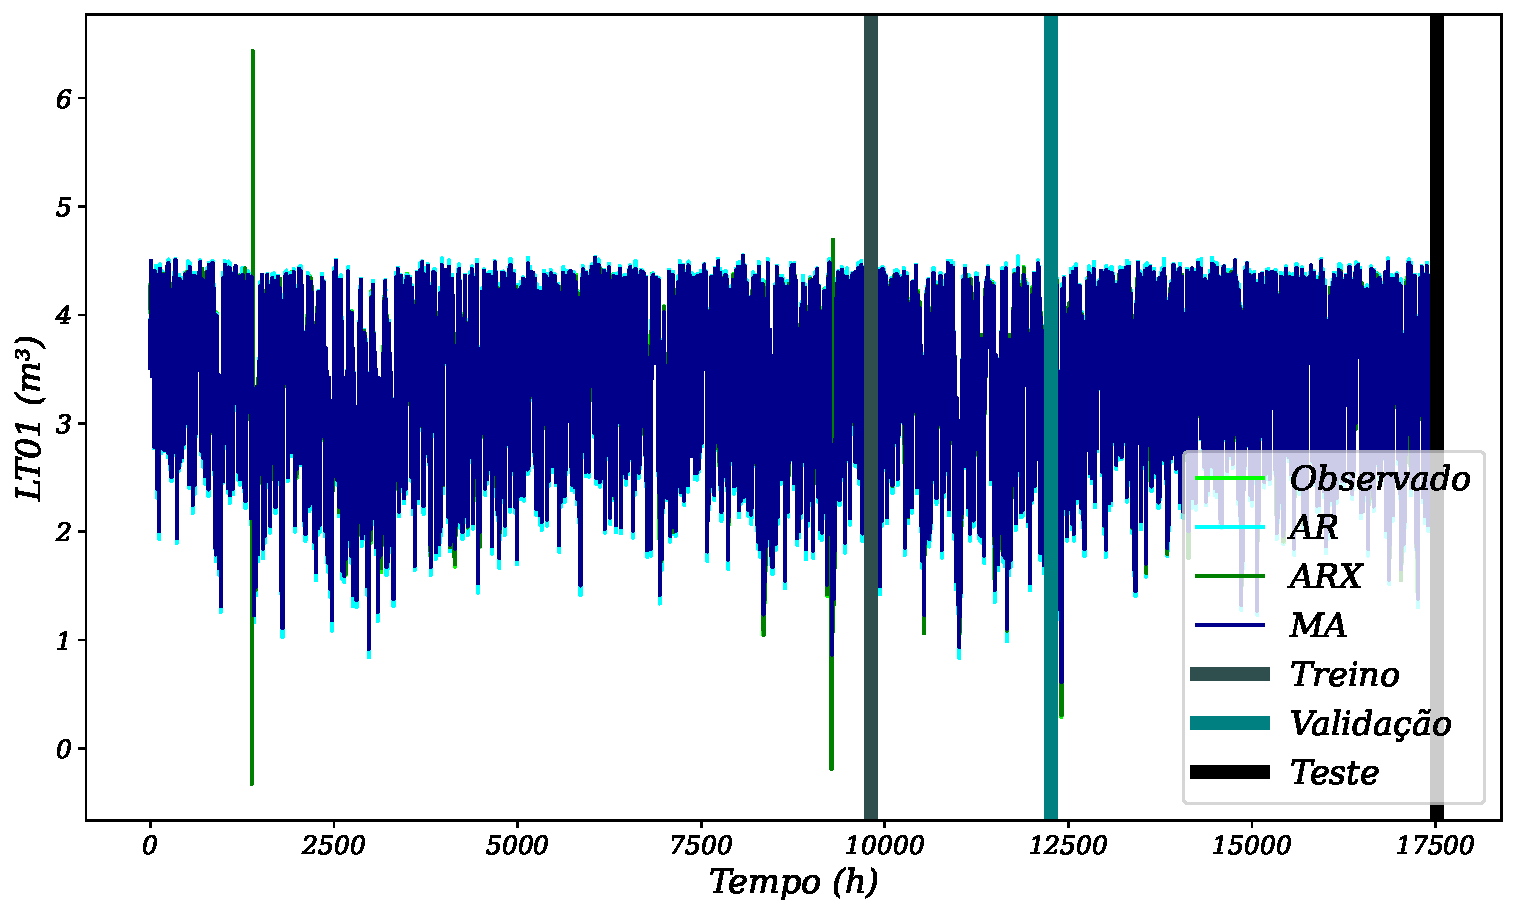
\includegraphics[width=0.7\linewidth]{Resultados/Figuras/1-AR-ARX-MA}
	
\end{figure}
\begin{figure}[!htb]
	\centering
	\caption{Comparação dos modelos de previsão ARIMAX, SARIMA e SARIMAX 1 passo à frente.}
	\label{fig:1-arimax-sarima-sarimax}
	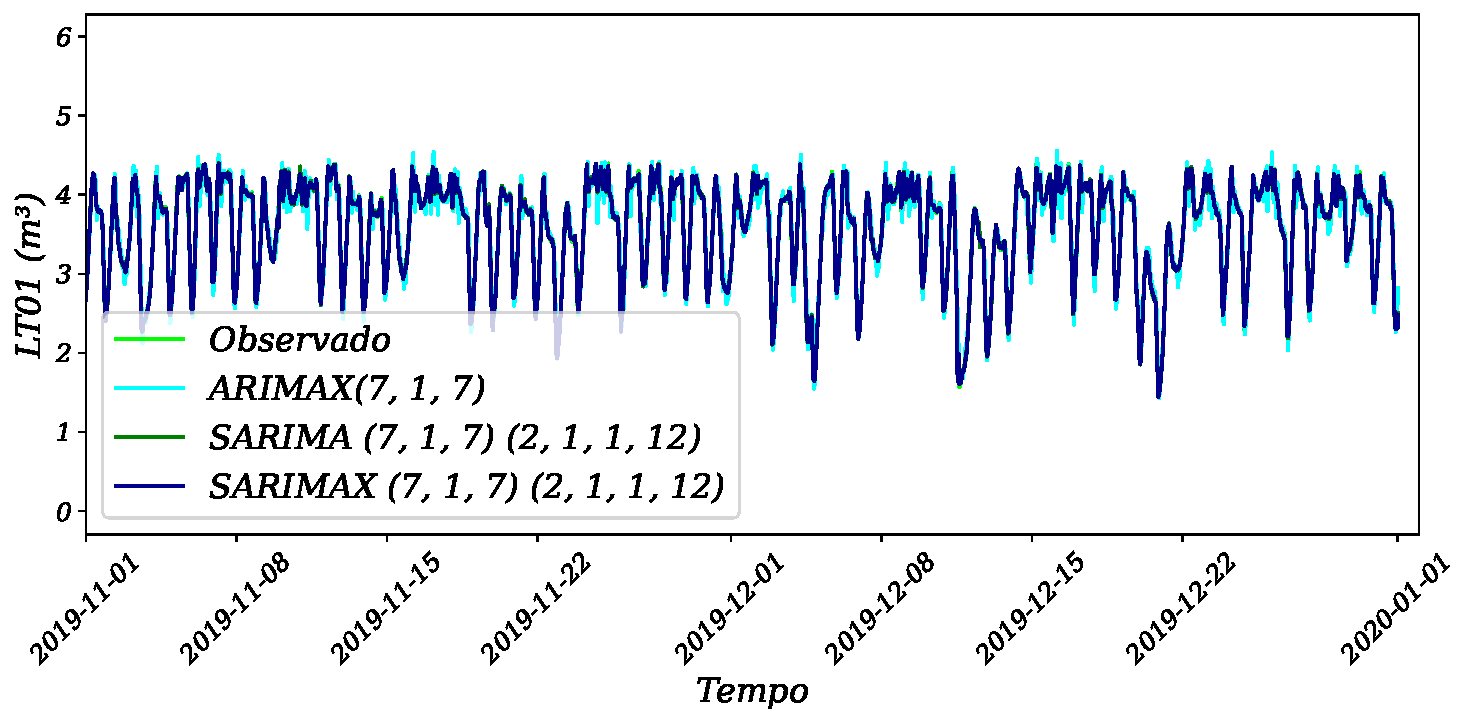
\includegraphics[width=0.7\linewidth]{Resultados/Figuras/1-ARIMAX-SARIMA-SARIMAX}
	
\end{figure}
\begin{figure}[!htb]
	\centering
	\caption{Comparação dos modelos de previsão ARMA e ARIMA 1 passo à frente.}
	\label{fig:1-arma-arima}
	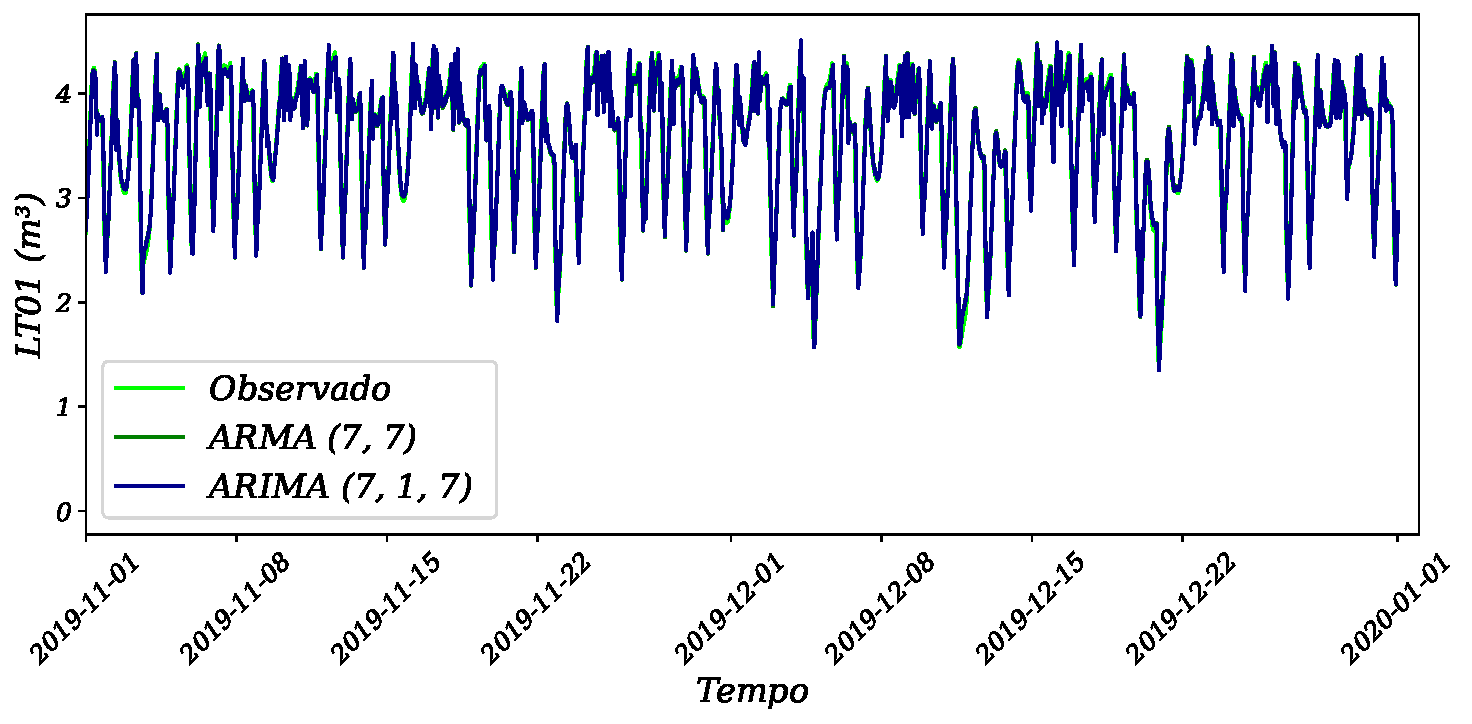
\includegraphics[width=0.7\linewidth]{Resultados/Figuras/1-ARMA-ARIMA}
	
\end{figure}
\begin{figure}[!htb]
	\centering
	\caption{Comparação dos modelos DT, RF, XGBoost e LightGBM 1 passo à frente.}
	\label{fig:lr-xgb-lgbm-rf}
	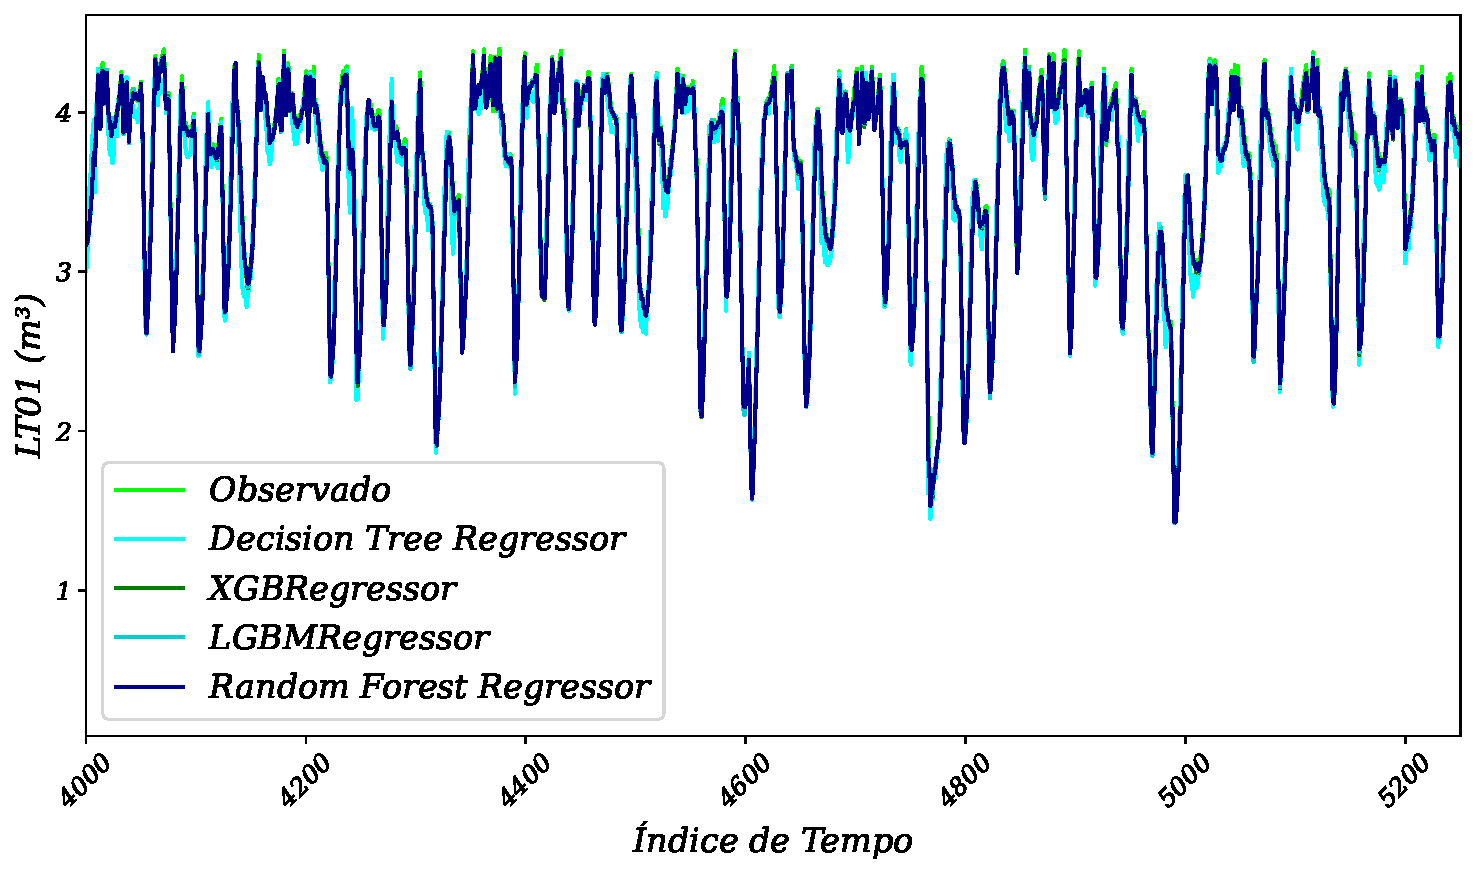
\includegraphics[width=0.7\linewidth]{Resultados/Figuras/LR-XGB-LGBM-RF}
	
\end{figure}
\begin{figure}[!htb]
	\centering
	\caption{Modelo de previsão RNN para vários horizontes de previsão.}
	\label{fig:rnn}
	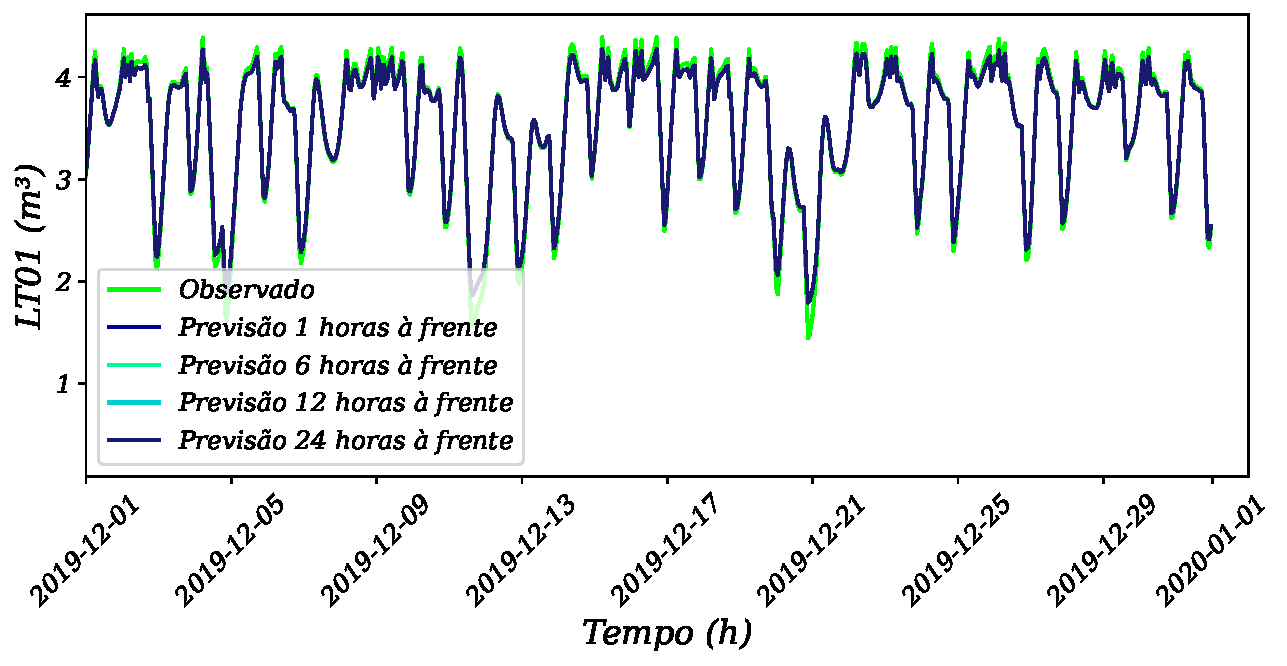
\includegraphics[width=0.9\linewidth]{Resultados/Figuras/RNN}
\end{figure}
\begin{figure}[!htb]
	\centering
	\caption{Previsões do modelo Prophet 24 passos à frente}\label{fig:prophet1}
	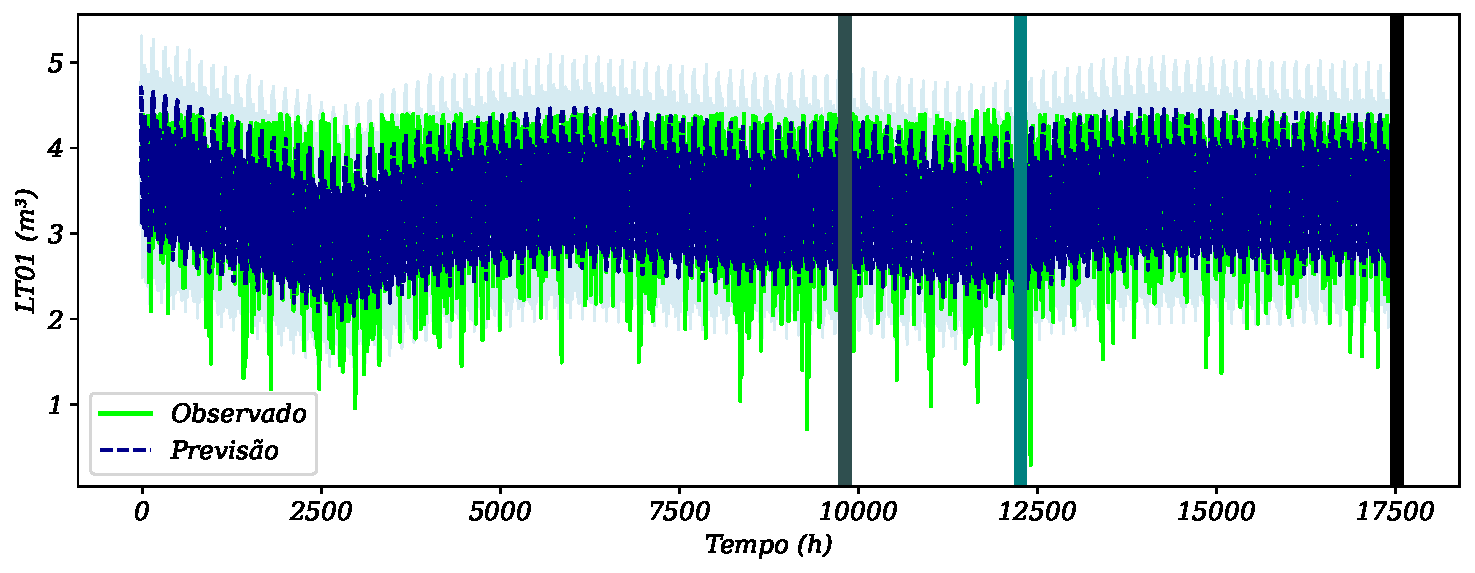
\includegraphics[width=0.9\linewidth]{Resultados/Figuras/prophet1}	
\end{figure}

\begin{landscape}
\begin{table}[!htb]
	\centering
	\setlength{\tabcolsep}{4pt} % Reduzir o espaçamento entre as colunas
	\caption{Comparação dos modelos de previsão através das métricas de desempenho para dados de treino.}\label{tb:apd-trn}
\begin{tabular}{llllllllllllllllllll}
	\hline
	Horizontes                         & Métricas & A    & B    & C    & D    & E    & F    & G    & H    & I    & J    & K    & L     & M    & N    & O   & P               & R    & S    \\ \hline
	\multirow{3}{*}{1 hora à frente}   & sMAPE    & 3,91 & 4,01 & 4,03 & 3,91 & 3,92 & 3,89 & 3,82 & 3,86 & 8,85 & 9,31 & 9,52 & 9,37  & 35,4 & 35,8 & 21  & \textbf{0,0665} & 23   & 23   \\ 
	& MAE      & 0,25 & 0,25 & 0,26 & 0,25 & 0,25 & 0,25 & 0,24 & 0,25 & 0,36 & 0,65 & 0,67 & 0,65  & 1,42 & 1,44 & 0,8 & \textbf{0,0023} & 0,83 & 0,83 \\  
	& RRMSE    & 0,09 & 0,10 & 0,09 & 0,09 & 0,09 & 0,09 & 0,09 & 0,09 & 0,21 & 0,21 & 0,21 & 0,21  & 2,3  & 0,65 & 0,8 & \textbf{0,0008} & 0,48 & 0,48 \\ \hline
	\multirow{3}{*}{6 horas à frente}  & sMAPE    & 9,97 & 10,1 & 9,7  & 9,98 & 9,97 & 10   & 10,1 & 9,99 & 6,99 & 12,4 & 12,7 & 9,369 & 66,2 & 83,9 & 34  & \textbf{0,0230} & 20,6 & 20,6 \\  
	& MAE      & 0,64 & 0,65 & 0,62 & 0,64 & 0,64 & 0,64 & 0,65 & 0,64 & 0,59 & 0,9  & 0,93 & 0,651 & 3,37 & 4,95 & 1,1 & \textbf{0,0007} & 0,72 & 0,72 \\  
	& RRMSE    & 0,23 & 0,23 & 0,23 & 0,23 & 0,23 & 0,23 & 0,23 & 0,23 & 0,16 & 0,32 & 0,33 & 0,209 & 5,02 & 1,71 & 1,2 & \textbf{0,0006} & 0,45 & 0,45 \\ \hline
	\multirow{3}{*}{12 horas à frente} & sMAPE    & 11,6 & 11,6 & 11,3 & 11,6 & 11,5 & 11,7 & 11,8 & 11,6 & 6,99 & 12,4 & 12,7 & 9,369 & 72   & 98,6 & 25  & \textbf{0,0683} & 29,2 & 29,2 \\  
	& MAE      & 0,75 & 0,75 & 0,74 & 0,75 & 0,75 & 0,76 & 0,77 & 0,75 & 0,59 & 0,9  & 0,93 & 0,651 & 3,83 & 6,69 & 0,8 & \textbf{0,0022} & 1,11 & 1,11 \\  
	& RRMSE    & 0,27 & 0,27 & 0,26 & 0,27 & 0,26 & 0,27 & 0,27 & 0,27 & 0,16 & 0,32 & 0,33 & 0,209 & 5,69 & 2,25 & 0,9 & \textbf{0,0009} & 0,55 & 0,55 \\ \hline
	\multirow{3}{*}{24 horas à frente} & sMAPE    & 6,77 & 6,85 & 6,67 & 6,77 & 6,69 & 6,82 & 6,86 & 6,82 & 6,99 & 12,4 & 12,7 & 9,369 & 74,4 & 104  & 6,6 & \textbf{0,2328} & 26,8 & 26,8 \\  
	& MAE      & 0,43 & 0,44 & 0,43 & 0,43 & 0,43 & 0,44 & 0,44 & 0,43 & 0,59 & 0,9  & 0,93 & 0,651 & 4,04 & 7,5  & 0,2 & \textbf{0,0079} & 1    & 1    \\ 
	& RRMSE    & 0,17 & 0,17 & 0,17 & 0,17 & 0,17 & 0,17 & 0,17 & 0,17 & 0,16 & 0,32 & 0,33 & 0,209 & 5,99 & 2,5  & 0,3 & \textbf{0,0024} & 0,52 & 0,52 \\ \hline
\end{tabular}
	
	\captionsetup{justification=centering} % Centralizar a legenda
	A - AR, B - ARX, C - MA, D - ARMA, E - ARIMA, F - SARIMA, G - ARIMAX, H - SARIMAX, I - DT, J - RF, K - XGBoost, L - LightGBM, M - LSTM, N - GRU, O - Prophet, \textbf{P - RNN}, R - CNN, S - MLP.

\end{table}

	
	\newpage
	
	\begin{table}[!htb]
		\centering
		\setlength{\tabcolsep}{4pt} % Reduzir o espaçamento entre as colunas
		\caption{Comparação dos modelos de previsão através das métricas de desempenho para dados de teste.}\label{tb:apd-tst}
\begin{tabular}{llllllllllllllllllll}
	\hline
	Horizontes                         & Métricas & A    & B    & C    & D    & E    & F    & G    & H    & I    & J    & K    & L     & M    & N    & O   & P               & R    & S    \\ \hline
	\multirow{3}{*}{1 hora à frente}   & sMAPE    & 3,93 & 4,15 & 3,99 & 3,93 & 3,92 & 3,91 & 4,16 & 4,16 & 7,76 & 8,46 & 8,68 & 8,45  & 15,6 & 15,9 & 18  & \textbf{0,0744} & 20,6 & 20,6 \\  
	& MAE      & 0,26 & 0,27 & 0,26 & 0,26 & 0,26 & 0,26 & 0,27 & 0,27 & 0,40 & 0,61 & 0,63 & 0,61  & 0,53 & 0,54 & 0,5 & \textbf{0,0024} & 0,76 & 0,76 \\ 
	& RRMSE    & 0,09 & 0,10 & 0,09 & 0,09 & 0,09 & 0,09 & 0,10 & 0,10 & 0,18 & 0,19 & 0,20 & 0,19  & 1,01 & 0,33 & 0,5 & \textbf{0,0029} & 0,5  & 0,5  \\ \hline
	\multirow{3}{*}{6 horas à frente}  & sMAPE    & 9,74 & 9,94 & 9,44 & 9,74 & 9,71 & 9,76 & 9,96 & 9,96 & 6,36 & 10,7 & 11   & 8,446 & 59,5 & 72,7 & 30  & \textbf{0,0308} & 17,3 & 17,3 \\  
	& MAE      & 0,65 & 0,66 & 0,63 & 0,65 & 0,65 & 0,65 & 0,66 & 0,66 & 0,56 & 0,8  & 0,82 & 0,609 & 2,97 & 4,04 & 0,9 & \textbf{0,0007} & 0,62 & 0,62 \\ 
	& RRMSE    & 0,23 & 0,23 & 0,22 & 0,23 & 0,23 & 0,23 & 0,23 & 0,23 & 0,14 & 0,28 & 0,29 & 0,191 & 4,9  & 1,42 & 1,1 & \textbf{0,0033} & 0,46 & 0,46 \\ \hline
	\multirow{3}{*}{12 horas à frente} & sMAPE    & 11,1 & 11,2 & 10,9 & 11,1 & 11,1 & 11,2 & 11,2 & 11,3 & 6,36 & 10,8 & 11   & 8,446 & 68,4 & 94,1 & 24  & \textbf{0,0745} & 18,8 & 18,8 \\  
	& MAE      & 0,74 & 0,75 & 0,73 & 0,74 & 0,74 & 0,75 & 0,75 & 0,75 & 0,56 & 0,8  & 0,82 & 0,609 & 3,67 & 6,31 & 0,8 & \textbf{0,0023} & 0,68 & 0,68 \\  
	& RRMSE    & 0,26 & 0,26 & 0,25 & 0,26 & 0,26 & 0,26 & 0,26 & 0,26 & 0,14 & 0,28 & 0,29 & 0,191 & 6,01 & 2,11 & 1   & \textbf{0,0032} & 0,48 & 0,48 \\ \hline
	\multirow{3}{*}{24 horas à frente} & sMAPE    & 6,15 & 6,34 & 6,08 & 6,15 & 6,14 & 6,24 & 6,36 & 6,37 & 6,36 & 10,7 & 11   & 8,446 & 71,5 & 102  & 5   & \textbf{0,2385} & 18,1 & 18,1 \\ 
	& MAE      & 0,4  & 0,41 & 0,4  & 0,4  & 0,4  & 0,41 & 0,42 & 0,42 & 0,56 & 0,8  & 0,83 & 0,609 & 3,92 & 7,36 & 0,2 & \textbf{0,0081} & 0,65 & 0,65 \\ 
	& RRMSE    & 0,16 & 0,16 & 0,16 & 0,16 & 0,16 & 0,16 & 0,16 & 0,16 & 0,14 & 0,28 & 0,29 & 0,191 & 6,42 & 2,43 & 0,2 & \textbf{0,0041} & 0,47 & 0,47 \\ \hline
\end{tabular}
	
		
		\captionsetup{justification=centering} % Centralizar a legenda
A - AR, B - ARX, C - MA, D - ARMA, E - ARIMA, F - SARIMA, G - ARIMAX, H - SARIMAX, I - DT, J - RF, K - XGBoost, L - LightGBM, M - LSTM, N - GRU, O - Prophet, P - RNN, R - CNN, S - MLP.
	\end{table}
	
	\newpage
	
	\begin{table}[!htb]
		\centering
		\setlength{\tabcolsep}{4pt} % Reduzir o espaçamento entre as colunas
		\caption{Comparação dos modelos de previsão através das métricas de desempenho para dados de validação.}\label{tb:apd-vld}
\begin{tabular}{llllllllllllllllllll}
	\hline
	Horizontes                         & Métricas & A    & B    & C    & D    & E    & F    & G    & H    & I    & J     & K     & L     & M    & N    & O   & P               & R    & S    \\ \hline
	\multirow{3}{*}{1 hora à frente}   & sMAPE    & 4,08 & 4,28 & 4,20 & 4,09 & 4,10 & 4,20 & 4,26 & 4,29 & 8,54 & 10,47 & 10,66 & 10,45 & 29,8 & 29,4 & 14  & \textbf{0,0675} & 18,3 & 18,3 \\  
	& MAE      & 0,25 & 0,26 & 0,26 & 0,25 & 0,25 & 0,26 & 0,26 & 0,26 & 0,32 & 0,72  & 0,74  & 0,72  & 1,1  & 1,08 & 0,5 & \textbf{0,0023} & 0,6  & 0,6  \\  
	& RRMSE    & 0,10 & 0,10 & 0,10 & 0,10 & 0,10 & 0,10 & 0,10 & 0,10 & 0,20 & 0,23  & 0,24  & 0,23  & 1,87 & 0,56 & 0,5 & \textbf{0,0008} & 0,39 & 0,39 \\ \hline
	\multirow{3}{*}{6 horas à frente}  & sMAPE    & 10,9 & 11,1 & 10,6 & 10,9 & 10,9 & 11   & 11,1 & 11,1 & 6,8  & 13,9  & 14,2  & 10,45 & 67,9 & 84   & 7,2 & \textbf{0,0229} & 20,5 & 20,5 \\ 
	& MAE      & 0,68 & 0,69 & 0,66 & 0,68 & 0,68 & 0,69 & 0,69 & 0,69 & 0,57 & 1,01  & 1,04  & 0,721 & 3,39 & 4,81 & 0,2 & \textbf{0,0007} & 0,69 & 0,69 \\ 
	& RRMSE    & 0,25 & 0,25 & 0,24 & 0,25 & 0,25 & 0,25 & 0,25 & 0,25 & 0,16 & 0,36  & 0,37  & 0,233 & 4,98 & 1,72 & 0,3 & \textbf{0,0005} & 0,44 & 0,44 \\ \hline
	\multirow{3}{*}{12 horas à frente} & sMAPE    & 12,7 & 12,8 & 12,4 & 12,7 & 12,6 & 12,8 & 12,8 & 12,8 & 6,8  & 13,9  & 14,2  & 10,45 & 74,4 & 100  & 15  & \textbf{0,0689} & 22,9 & 22,9 \\  
	& MAE      & 0,8  & 0,81 & 0,79 & 0,8  & 0,8  & 0,81 & 0,81 & 0,81 & 0,57 & 1,01  & 1,04  & 0,721 & 3,92 & 6,71 & 0,5 & \textbf{0,0022} & 0,79 & 0,79 \\  
	& RRMSE    & 0,29 & 0,29 & 0,28 & 0,29 & 0,29 & 0,29 & 0,29 & 0,29 & 0,16 & 0,36  & 0,37  & 0,233 & 5,73 & 2,33 & 0,6 & \textbf{0,0008} & 0,48 & 0,48 \\ \hline
	\multirow{3}{*}{24 horas à frente} & sMAPE    & 7,3  & 7,45 & 7,19 & 7,3  & 7,27 & 7,37 & 7,43 & 7,46 & 6,8  & 13,9  & 14,2  & 10,45 & 76,9 & 106  & 13  & \textbf{0,2342} & 22,9 & 22,9 \\  
	& MAE      & 0,46 & 0,46 & 0,45 & 0,46 & 0,45 & 0,46 & 0,46 & 0,46 & 0,57 & 1,01  & 1,04  & 0,721 & 4,14 & 7,59 & 0,4 & \textbf{0,0077} & 0,79 & 0,79 \\  
	& RRMSE    & 0,18 & 0,18 & 0,18 & 0,18 & 0,18 & 0,18 & 0,18 & 0,18 & 0,16 & 0,36  & 0,37  & 0,233 & 6,04 & 2,61 & 0,6 & \textbf{0,0024} & 0,48 & 0,48 \\ \hline
\end{tabular}

		
		\captionsetup{justification=centering} % Centralizar a legenda
	A - AR, B - ARX, C - MA, D - ARMA, E - ARIMA, F - SARIMA, G - ARIMAX, H - SARIMAX, I - DT, J - RF, K - XGBoost, L - LightGBM, M - LSTM, N - GRU, O - Prophet, P - RNN, R - CNN, S - MLP.
	\end{table}
	
	\newpage
	
	\begin{table}[!htb]
		\centering
		\setlength{\tabcolsep}{4pt} % Reduzir o espaçamento entre as colunas
		\caption{Comparação dos modelos de previsão através das métricas de desempenho para todos dados}\label{tb:apd-int}
	\begin{tabular}{llllllllllllllllllll}
		\hline
		Horizontes                         & Métricas & A    & B    & C    & D    & E    & F    & G    & H    & I    & J    & K    & L     & M    & N    & O   & P               & R    & S    \\ \hline
		\multirow{3}{*}{1 hora à frente}   & sMAPE    & 3,94 & 4,08 & 4,05 & 3,93 & 3,95 & 3,91 & 4,05 & 4,05 & 8,51 & 9,22 & 9,43 & 9,244 & 17,1 & 17,4 & 17  & \textbf{0,0690} & 22,5 & 22,5 \\  
		& MAE      & 0,25 & 0,26 & 0,26 & 0,25 & 0,25 & 0,25 & 0,26 & 0,26 & 0,36 & 0,65 & 0,67 & 0,648 & 0,57 & 0,58 & 0,5 & \textbf{0,0023} & 0,81 & 0,81 \\  
		& RRMSE    & 0,09 & 0,1  & 0,09 & 0,09 & 0,09 & 0,09 & 0,1  & 0,1  & 0,2  & 0,21 & 0,21 & 0,207 & 1,01 & 0,31 & 0,5 & \textbf{0,0017} & 0,49 & 0,49 \\ \hline
		\multirow{3}{*}{6 horas à frente}  & sMAPE    & 10   & 10,2 & 9,75 & 10   & 10   & 10,1 & 10,2 & 10,1 & 6,77 & 12,1 & 12,4 & 12,07 & 61,7 & 74,6 & 30  & \textbf{0,0253} & 20   & 20   \\  
		& MAE      & 0,65 & 0,66 & 0,63 & 0,65 & 0,65 & 0,65 & 0,66 & 0,65 & 0,58 & 0,89 & 0,91 & 0,885 & 3,04 & 4,08 & 0,9 & \textbf{0,0007} & 0,7  & 0,7  \\ 
		& RRMSE    & 0,23 & 0,23 & 0,23 & 0,23 & 0,23 & 0,23 & 0,23 & 0,23 & 0,16 & 0,32 & 0,32 & 0,316 & 4,65 & 1,45 & 1   & \textbf{0,0019} & 0,46 & 0,46 \\ \hline
		\multirow{3}{*}{12 horas à frente} & sMAPE    & 11,6 & 11,7 & 11,4 & 11,6 & 11,6 & 11,7 & 11,8 & 11,7 & 6,77 & 12,1 & 12,4 & 12,12 & 70,7 & 96   & 25  & \textbf{0,0703} & 28,7 & 28,7 \\  
		& MAE      & 0,76 & 0,76 & 0,74 & 0,76 & 0,75 & 0,76 & 0,77 & 0,76 & 0,58 & 0,89 & 0,91 & 0,889 & 3,75 & 6,38 & 0,8 & \textbf{0,0023} & 1,09 & 1,09 \\  
		& RRMSE    & 0,27 & 0,27 & 0,26 & 0,27 & 0,27 & 0,27 & 0,27 & 0,27 & 0,16 & 0,32 & 0,32 & 0,317 & 5,69 & 2,16 & 1   & \textbf{0,0019} & 0,56 & 0,56 \\ \hline
		\multirow{3}{*}{24 horas à frente} & sMAPE    & 6,66 & 6,79 & 6,57 & 6,66 & 6,6  & 6,71 & 6,82 & 6,8  & 6,77 & 12,1 & 12,4 & 12,21 & 73,8 & 104  & 4,7 & \textbf{0,2347} & 26,2 & 26,2 \\  
		& MAE      & 0,43 & 0,43 & 0,42 & 0,43 & 0,42 & 0,43 & 0,44 & 0,43 & 0,58 & 0,89 & 0,92 & 0,897 & 4,01 & 7,44 & 0,2 & \textbf{0,0080} & 0,98 & 0,98 \\ 
		& RRMSE    & 0,17 & 0,17 & 0,17 & 0,17 & 0,17 & 0,17 & 0,17 & 0,17 & 0,16 & 0,32 & 0,32 & 0,319 & 6,07 & 2,49 & 0,2 & \textbf{0,0030} & 0,53 & 0,53 \\ \hline
	\end{tabular}

		
		\captionsetup{justification=centering} % Centralizar a legenda
		A - AR, B - ARX, C - MA, D - ARMA, E - ARIMA, F - SARIMA, G - ARIMAX, H - SARIMAX, I - DT, J - RF, K - XGBoost, L - LightGBM, M - LSTM, N - GRU, O - Prophet, P - RNN, R - CNN, S - MLP.
	\end{table}
\end{landscape}

Na Tabela \ref{tab:metrics} são mostrados os valores das métricas estatísticas para todos os modelos de previsão para 24 passos à frente (1 dia) usando todos os dados.

\begin{table}[!htb]
	\centering
	\caption{Métricas de avaliação dos modelos com 24 passos à frente.}
	\label{tab:metrics}


	
	\begin{tabular}{llll}
		\hline
		\text{Modelo} & \text{sMAPE} & \text{MAE} & \text{RRMSE} \\
		\hline
		Prophet & 4,74 & 0,15 & 0,18 \\
		MLP & 26,22 & 0,980 & 0,531 \\
		CNN & 26,22 & 0,980 & 0,531 \\
		\textbf{RNN} & \textbf{0,235} & \textbf{0,008} & \textbf{0,003} \\
		LSTM & 73,75 & 4,010 & 6,068 \\
		GRU & 103,57 & 7,443 & 2,485 \\
		AR & 6,66 & 0,428 & 0,169 \\
		ARX & 6,79 & 0,434 & 0,173 \\
		MA & 6,57 & 0,423 & 0,166 \\
		ARMA & 6,66 & 0,428 & 0,169 \\
		ARIMA & 6,60 & 0,424 & 0,167 \\
		SARIMA & 6,71 & 0,432 & 0,170 \\
		ARIMAX & 6,82 & 0,436 & 0,173 \\
		SARIMAX & 6,80 & 0,435 & 0,173 \\
		DT & 6,77 & 0,577 & 0,158 \\
		RF & 12,09 & 0,886 & 0,316 \\
		XGBoost & 12,41 & 0,916 & 0,323 \\
		LigthGBM & 12,21 & 0,897 & 0,319 \\
		\hline
	\end{tabular}
\end{table}

Na tabela prévia os diversos modelos de previsão de séries temporais foram avaliados para horizonte de previsão de $24$ horas. Para cada métrica sMAPE, MAE, e RRMSE, identificou-se o modelo que apresentou o menor valor. A métrica sMAPE apontou que o modelo RNN obteve o menor valor. Quanto à métrica MAE, novamente o modelo RNN demonstrou o menor valor e com a métrica RRMSE também.

Para validar estatisticamente as diferenças entre os modelos, foi realizado um teste estatístico denominado Teste de Friedman. Esse teste avalia o desempenho dos modelos em todas as métricas simultaneamente. O resultado do teste de Friedman revelou evidências estatísticas que pelo menos um dos modelos apresenta superioridade estatística em relação aos demais, considerando um nível de significância de $0.05$.



\subsection{Teste de Signific\^ancia}

O teste de Friedman e o teste de Nemenyi são usados para comparar os modelos de previsão. O teste de Nemenyi é uma ferramenta de comparação múltipla frequentemente empregada após a aplicação de testes não paramétricos com três ou mais fatores.

Usando os resultados obtidos na Tabela \ref{tb:nemenyi} para calcular o teste de Nemenyi, em comparação aos modelos que foram previstos, no teste Nemenyi. Nesse teste, em comparação com os modelos, calcula-se entre as métricas estatísticas qual desses modelos contém o menor valor de p. Dentro de todos os modelos de previsão, o RNN foi o modelo que obteve o menor valor registrado nas métricas estatísticas.

O teste de Friedman, com um valor de estatística de teste de $105.016$ e um valor de p $0$, indica que existem evidências estatísticas sugerindo que, pelo menos, um dos modelos (ou todos) apresenta um desempenho significativamente diferente dos demais. O valor extremamente baixo de p, próximo de zero, sugere que as diferenças observadas não são simplesmente devido ao acaso. Portanto, há uma diferença estatisticamente significativa entre os grupos testados.

No contexto do estudo, os resultados da análise comparativa revelaram diferenças estatisticamente significativas entre vários pares de modelos, conforme indicado pelas entradas da Tabela \ref{tb:nemenyi}. Isso sugere que pelo menos um modelo é considerado estatisticamente superior aos demais, com base nas comparações realizadas. Por exemplo, o modelo que tem o menor valor de p entre esses modelos é o da coluna C (MA) na linha L (RF), com um valor de $0,097$, o que significa que os dois modelos têm diferença estatisticamente significativa.



\begin{table}[!htb]
	\caption{Teste de significância Nemenyi}\label{tb:nemenyi}
	\centering
	\small
	\setlength{\tabcolsep}{4pt} % Reduzir o espaçamento entre as colunas
\begin{tabular}{@{}lllllllllllll@{}}
	\toprule
	\textbf{Modelo} & \textbf{A} & \textbf{B} & \textbf{C}     & \textbf{D} & \textbf{E} & \textbf{F} & \textbf{G} & \textbf{H} & \textbf{I} & \textbf{J} & \textbf{K} & \textbf{L} \\ \midrule
	\textbf{A}       & 1          & 0,9        & 0,9            & 0,9        & 0,9        & 0,9        & 0,9        & 0,9        & 0,9        & 0,9        & 0,9        & 0,877      \\
	\textbf{B}       & 0,9        & 1          & 0,9            & 0,9        & 0,9        & 0,9        & 0,9        & 0,9        & 0,693      & 0,693      & 0,9        & 0,442      \\
	\textbf{C}       & 0,9        & 0,9        & 1              & 0,9        & 0,785      & 0,9        & 0,9        & 0,9        & 0,253      & 0,253      & 0,816      & 0,097      \\
	\textbf{D}       & 0,9        & 0,9        & 0,9            & 1          & 0,9        & 0,9        & 0,9        & 0,9        & 0,754      & 0,754      & 0,9        & 0,508      \\
	\textbf{E}       & 0,9        & 0,9        & 0,785          & 0,9        & 1          & 0,877      & 0,9        & 0,9        & 0,9        & 0,9        & 0,9        & 0,9        \\
	\textbf{F}       & 0,9        & 0,9        & 0,9            & 0,9        & 0,877      & 1          & 0,9        & 0,9        & 0,340      & 0,340      & 0,9        & 0,143      \\
	\textbf{G}       & 0,9        & 0,9        & 0,9            & 0,9        & 0,9        & 0,9        & 1          & 0,9        & 0,9        & 0,9        & 0,9        & 0,877      \\
	\textbf{H}       & 0,9        & 0,9        & 0,9            & 0,9        & 0,9        & 0,9        & 0,9        & 1          & 0,9        & 0,9        & 0,9        & 0,877      \\
	\textbf{I}       & 0,9        & 0,693      & 0,253          & 0,754      & 0,9        & 0,340      & 0,9        & 0,9        & 1          & 0,9        & 0,9        & 0,9        \\
	\textbf{J}       & 0,9        & 0,693      & 0,253          & 0,754      & 0,9        & 0,340      & 0,9        & 0,9        & 0,9        & 1          & 0,9        & 0,9        \\
	\textbf{K}       & 0,9        & 0,9        & 0,816          & 0,9        & 0,9        & 0,9        & 0,9        & 0,9        & 0,9        & 0,9        & 1          & 0,9        \\
	\textbf{L}       & 0,877      & 0,442      & \textbf{0,097} & 0,508      & 0,9        & 0,143      & 0,877      & 0,877      & 0,9        & 0,9        & 0,9        & 1          \\ \bottomrule
\end{tabular}
	
	AR - A,	ARX	- B, MA	- C,ARMA - D, ARIMA - E, SARIMA - F, SARIMAX - G, ARIMAX	- H, DT	- I, XGBoost - J, LightGBM - K, RF - L.
	
\end{table}


O valor crítico CD foi utilizado para determinar se dois modelos eram significativamente diferentes entre si. Esse valor é calculado com base no valor crítico obtido da Tabela \ref{tb:nemenyi} de teste de Nemenyi, o número de modelos e o número total de amostras. O valor CD é uma métrica que auxilia na interpretação das diferenças entre os modelos, ajudando a identificar quais pares de modelos apresentam diferenças estatisticamente significativas.

Os resultados da pesquisa indicam a existência de evidências estatísticas que sugerem a superioridade de pelo menos um modelo em relação aos demais. A análise de comparação significativa entre os modelos revelou pares de modelos que apresentam diferenças estatisticamente significativas em seus desempenhos, conforme exibido na Tabela \ref{tb:nemenyi}, onde cada valor com três casas decimais após a vírgula representa modelos que têm significância estatística entre si.

Na Tabela \ref{tb:nemeyirede} é determinado quais modelos apresentam diferenças estatisticamente significativas entre si, foi conduzido o teste de comparações múltiplas de Nemenyi. Esse teste avalia todos os pares possíveis de modelos e identifica quais deles possuem diferenças estatisticamente significativas. O modelo RNN apresentou o menor erro nas métricas mas em questão de diferenças significativas ao analisar em relação aos modelos LSTM, GRU e os demais, não demonstra tanta diferença em comparação com os modelos que foi calculado entre eles, sendo o valor critico do RNN o mais baixo foi relacionado com o modelo CNN.

No teste de Friedman, a estatística de teste mostrou um valor de $19,117$, enquanto o valor de p foi calculado como $0,0018$. Devido a esses valores baixos, o resultado da correlação desse teste não indica tanta evidência estatística.

\begin{table}[!htb]
	\caption{Teste de significância Nemenyi dos modelos LSTM, GRU, RNN, CNN, MLP e Prophet.}\label{tb:nemeyirede}
	\centering
\begin{tabular}{@{}lllllll@{}}
	\toprule
	\textbf{Modelo} & \textbf{LSTM} & \textbf{GRU} & \textbf{RNN} & \textbf{CNN} & \textbf{MLP} & \textbf{Prophet} \\ \midrule
	\textbf{LSTM}    & 1             & 0,9          & 0,170        & 0,9          & 0,9          & 0,170            \\
	\textbf{GRU}     & 0,9           & 1            & 0,170        & 0,9          & 0,9          & 0,170            \\
	\textbf{RNN}     & 0,170         & 0,170        & 1            & 0,352        & 0,170        & 0,9              \\
	\textbf{CNN}     & 0,9           & 0,9          & 0,352        & 1            & 0,9          & 0,352            \\
	\textbf{MLP}     & 0,9           & 0,9          & 0,170        & 0,9          & 1            & 0,170            \\
	\textbf{Prophet} & 0,170         & 0,170        & 0,9          & 0,352        & 0,170        & 1                \\ \bottomrule
\end{tabular}
\end{table}





\subsubsection{Compara\c c\~ao dos Modelos}

Com o objetivo de obter uma análise mais aprofundada do desempenho de cada modelo, foi realizada uma comparação por meio de um gráfico de violino e de barra. Dessa forma, pôde-se observar qual dos modelos apresentava o melhor desempenho.

Ao examinar os modelos representados nas Figuras \ref{fig:modelos-arima} e \ref{fig:violin-lr-xgb-lgbm-rf}, identifico os modelos que se destacam em relação à natureza dos dados. Na Figura \ref{fig:basic_comparar}, que compara os modelos ARIMA e XGBoost com outros, torna-se evidente que os modelos ARIMA como AR, ARX, MA, ARMA, ARIMAX e SARIMAX demonstram um desempenho sólido. Os modelos baseados em gradientes e regressão, como o XGBoost, exibem resultados comparáveis, as redes neurais com o modelo Prophet, é importante destacar que os modelos de redes neurais, incluindo RNN, LSTM, GRU, MLP e CNN, foram avaliados em conjunto com o modelo Prophet. A análise das métricas demonstrou que o modelo RNN se sobressai como o vencedor entre as métricas avaliadas. Essa conclusão é respaldada pelas evidências de que pelo menos um modelo é superior aos demais. Os modelos com valores de valor de p abaixo de $0,05$ foram realçados em \textbf{negrito} para enfatizar sua significância. Beneficiando-se da otimização por meio do Optuna, uma abordagem de bayesiana usando o metodo TPE.


\begin{figure}[!htb]
	\centering
	\caption{Comparação dos modelos ARIMA.}\label{fig:modelos-arima}
	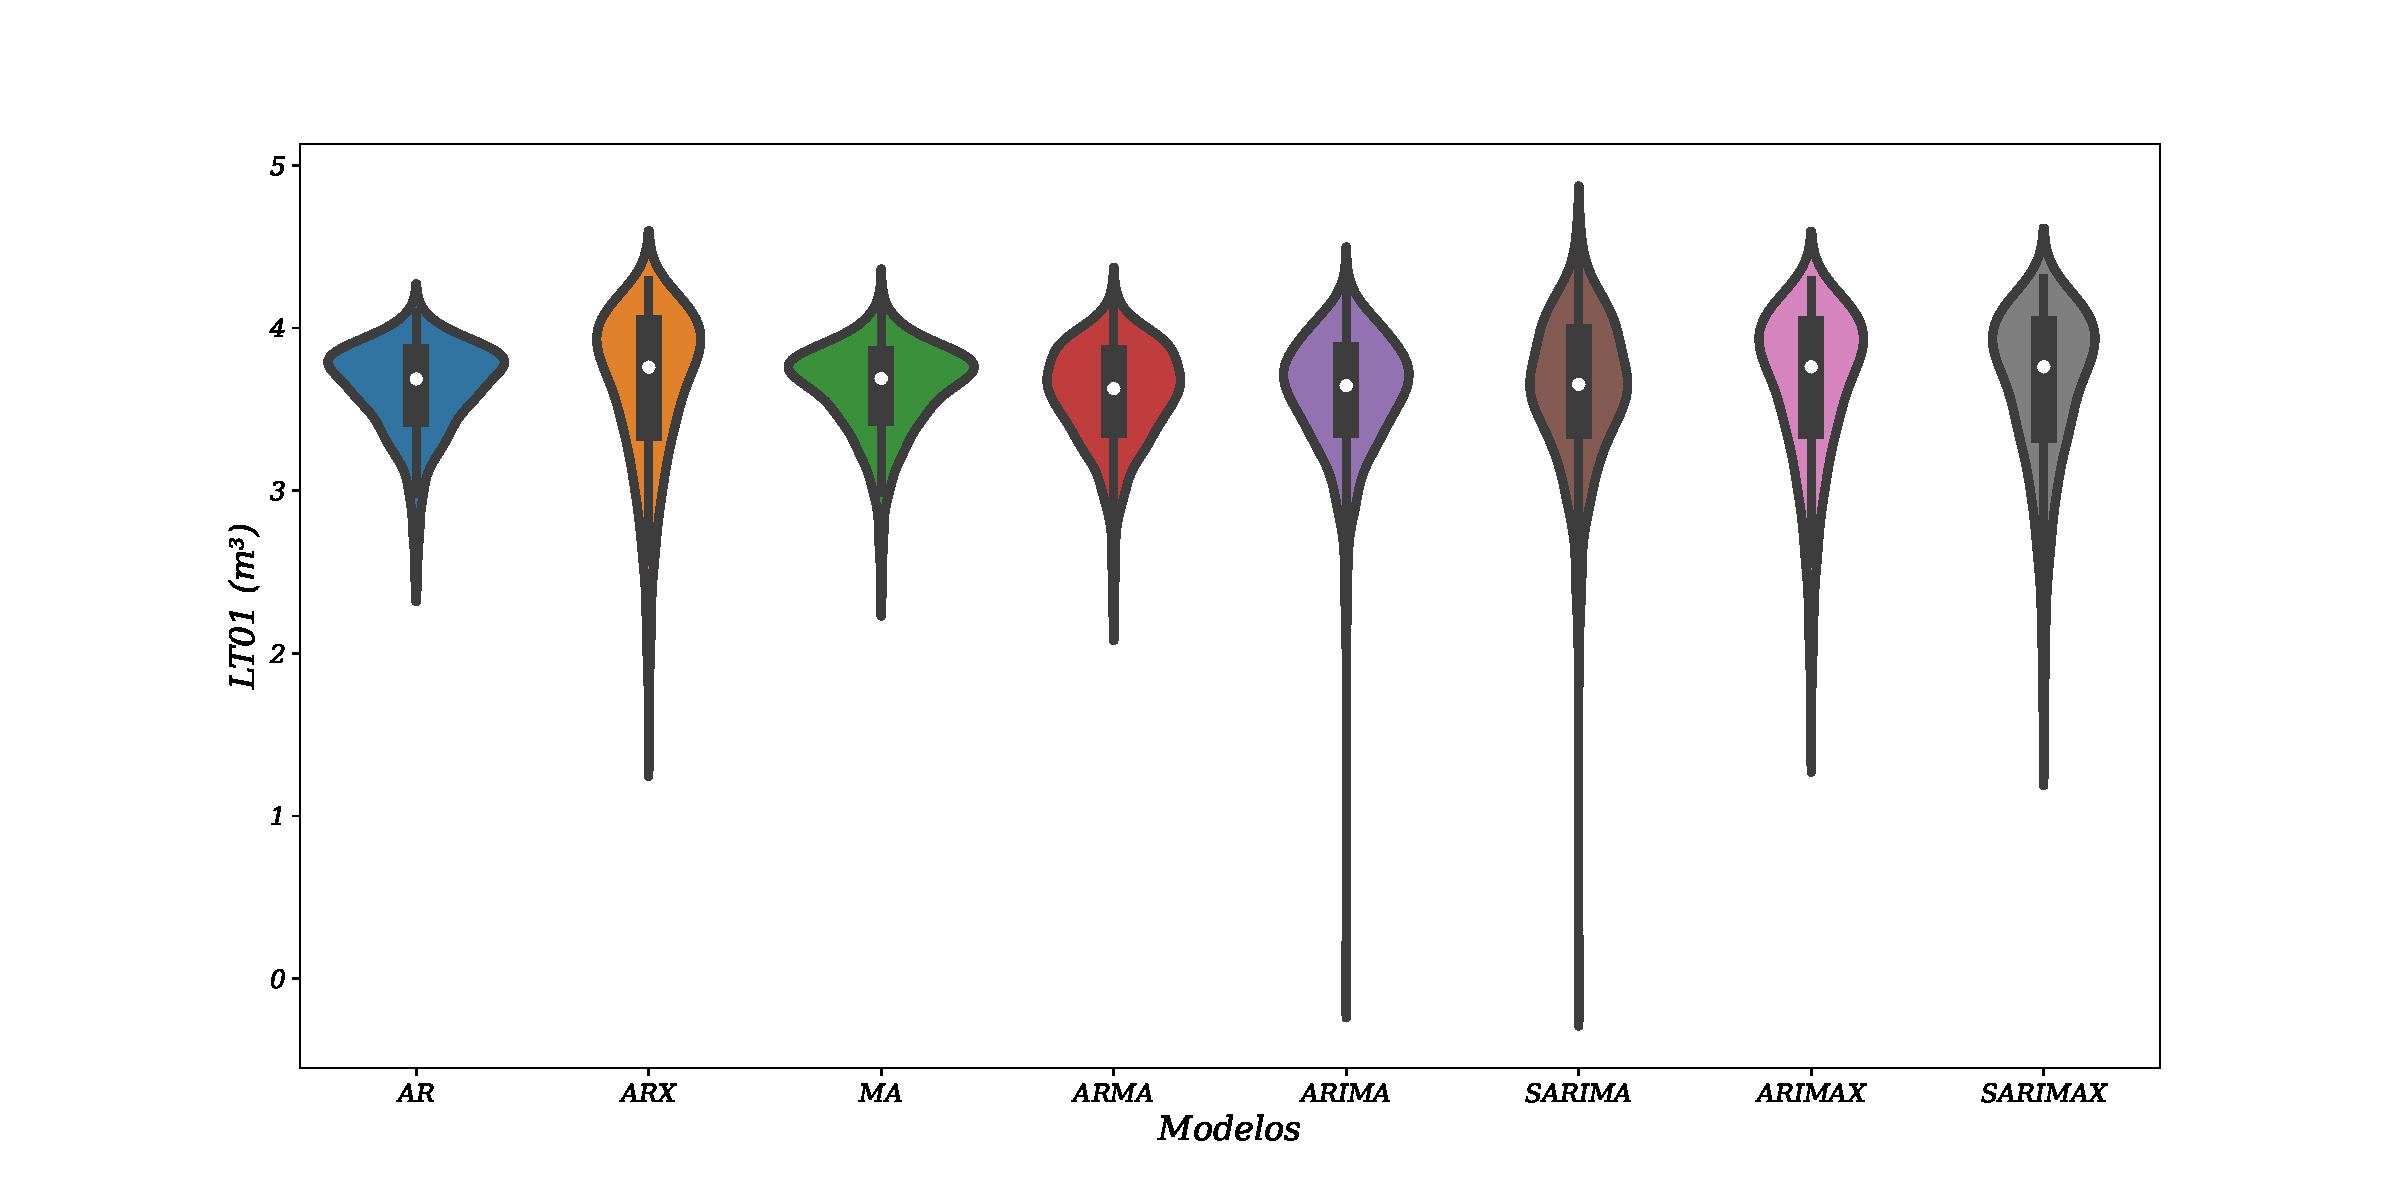
\includegraphics[width=\linewidth]{Resultados/Figuras/modelos-arima}
	
	
\end{figure}

Na Figura \ref{fig:violin-lr-xgb-lgbm-rf}, é feita uma comparação entre os modelos de gradiente e regressor. Esses modelos, por serem mais robustos e utilizar técnicas de otimização mais avançadas, mostram-se superiores aos modelos comparados. O modelo XGBoost, em particular, é identificado como superior em relação aos outros modelos na análise.

\begin{figure}[!htb]
	\centering
	\caption{Comparação de modelos de regressão}\label{fig:violin-lr-xgb-lgbm-rf}
	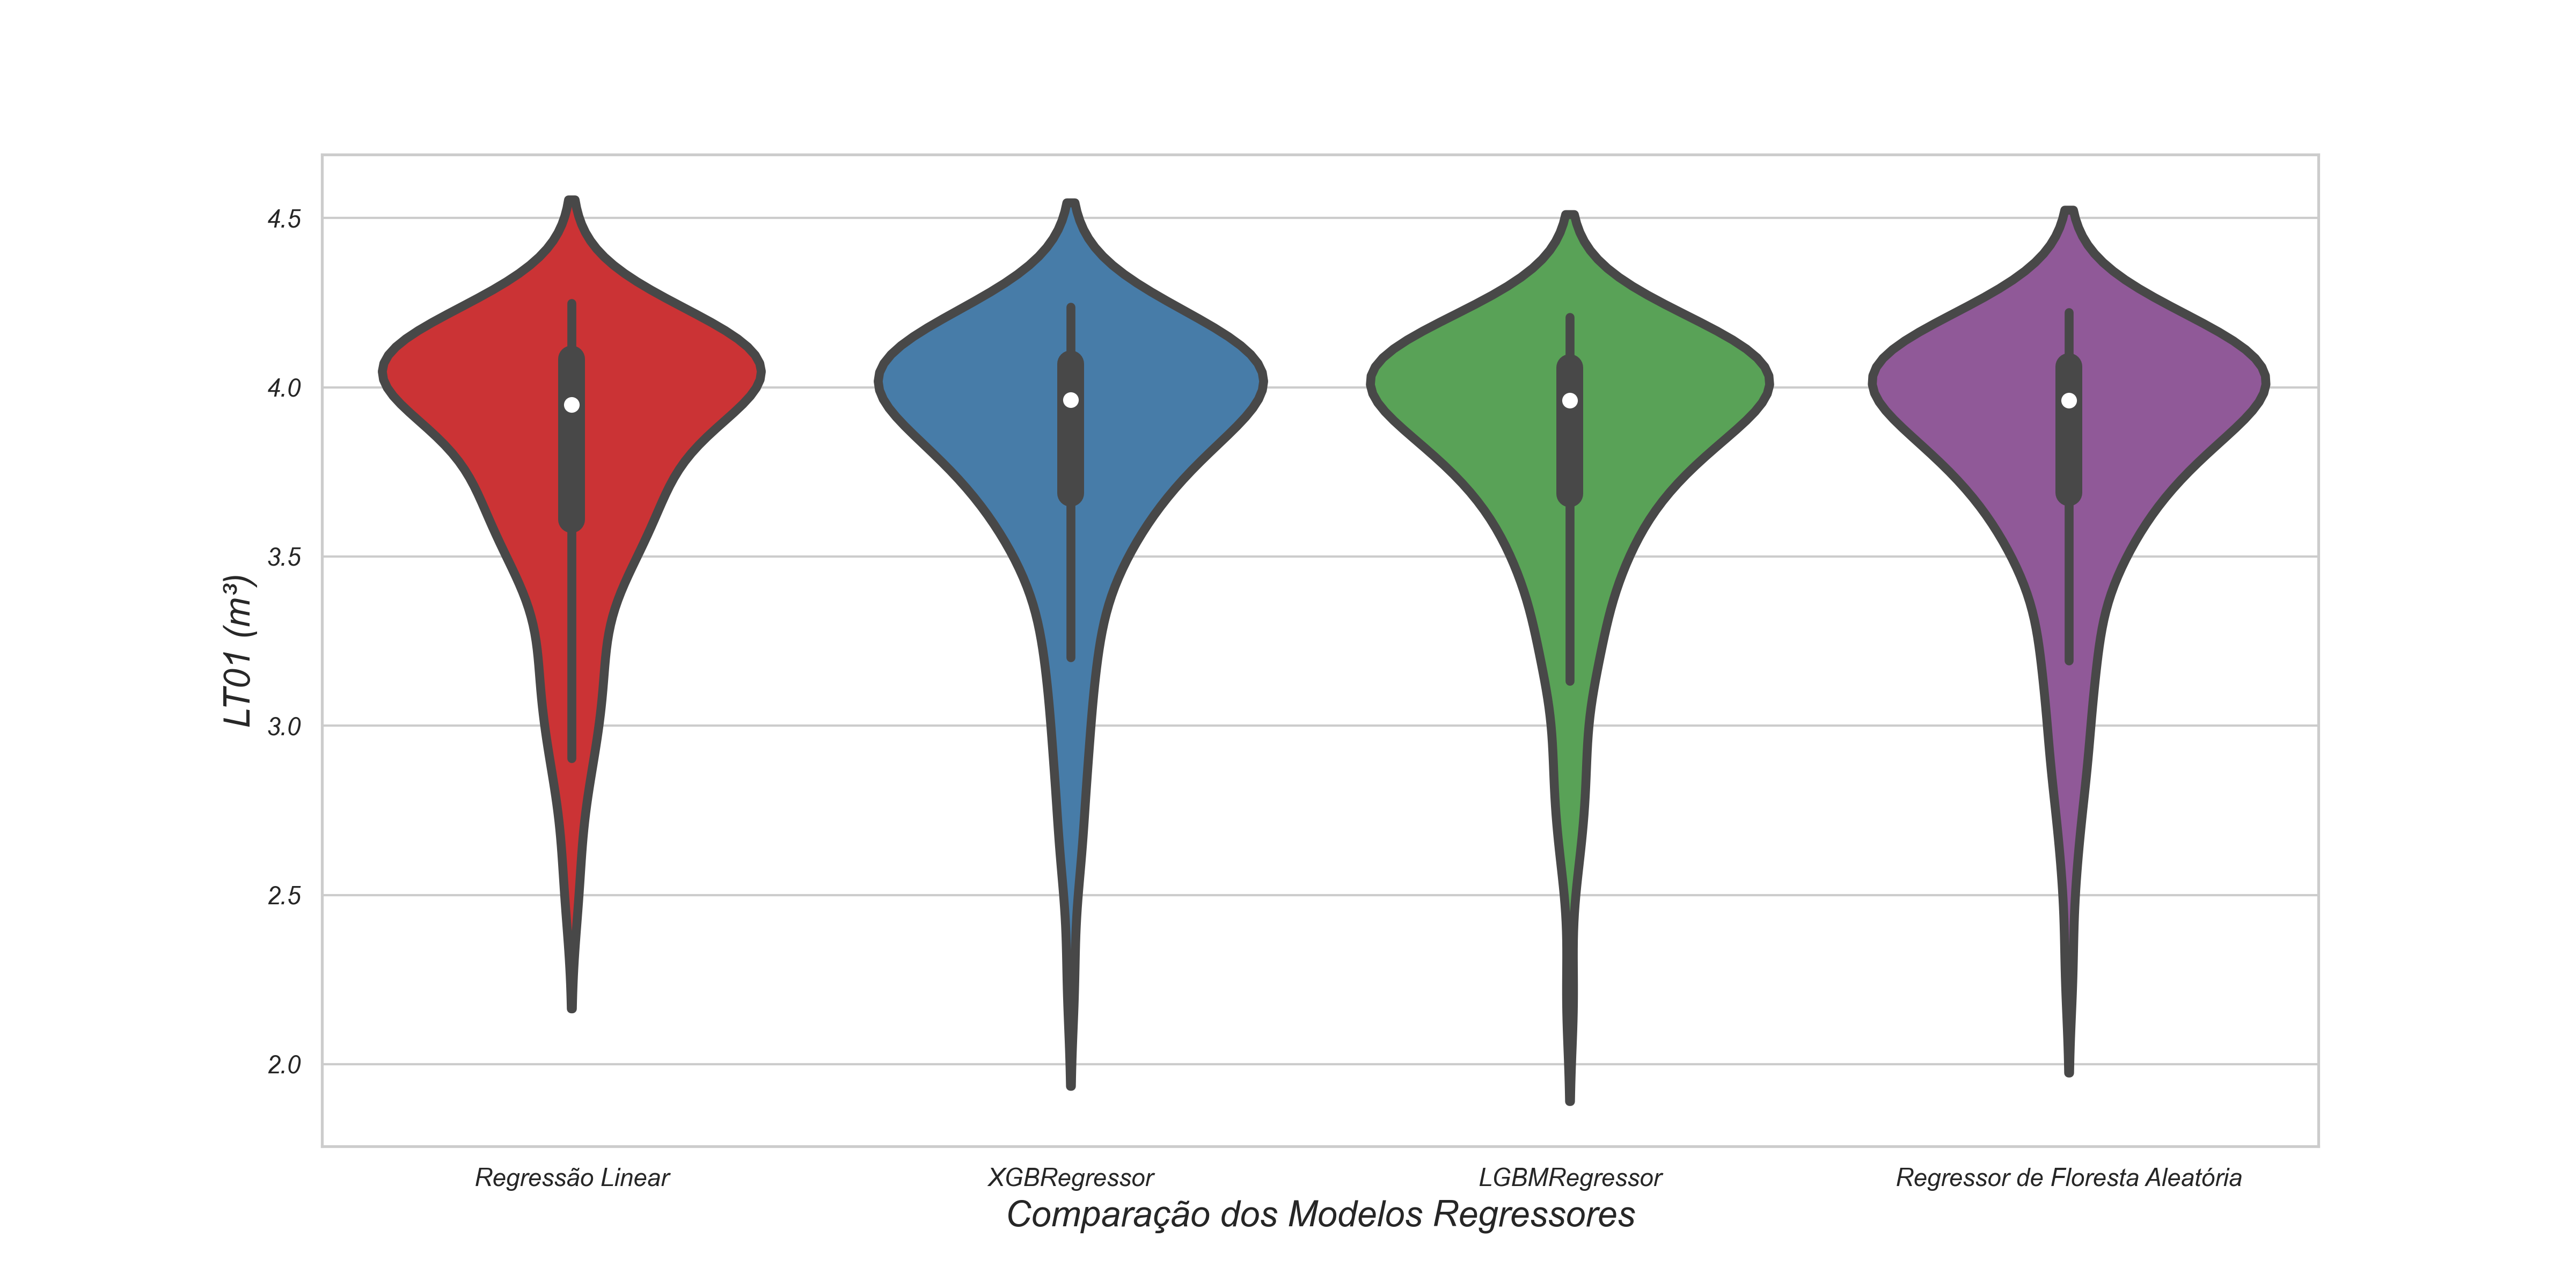
\includegraphics[width=\linewidth]{Resultados/Figuras/violin-LR-XGB-LGBM-RF}
	
\end{figure}

Na Figura \ref{fig:basic_comparar}, nota-se que todos os modelos trabalhados aqui, exceto o modelo LR, foram comparados em relação às métricas de desempenho. Mesmo sendo muito robustos, esses modelos não conseguiram obter um resultado tão bom quanto o RNN.


\begin{figure}[!htb]
	\centering
	\caption{Comparação dos modelos nas métricas sMAPE, MAE e RRMSE\label{fig:basic_comparar}}
	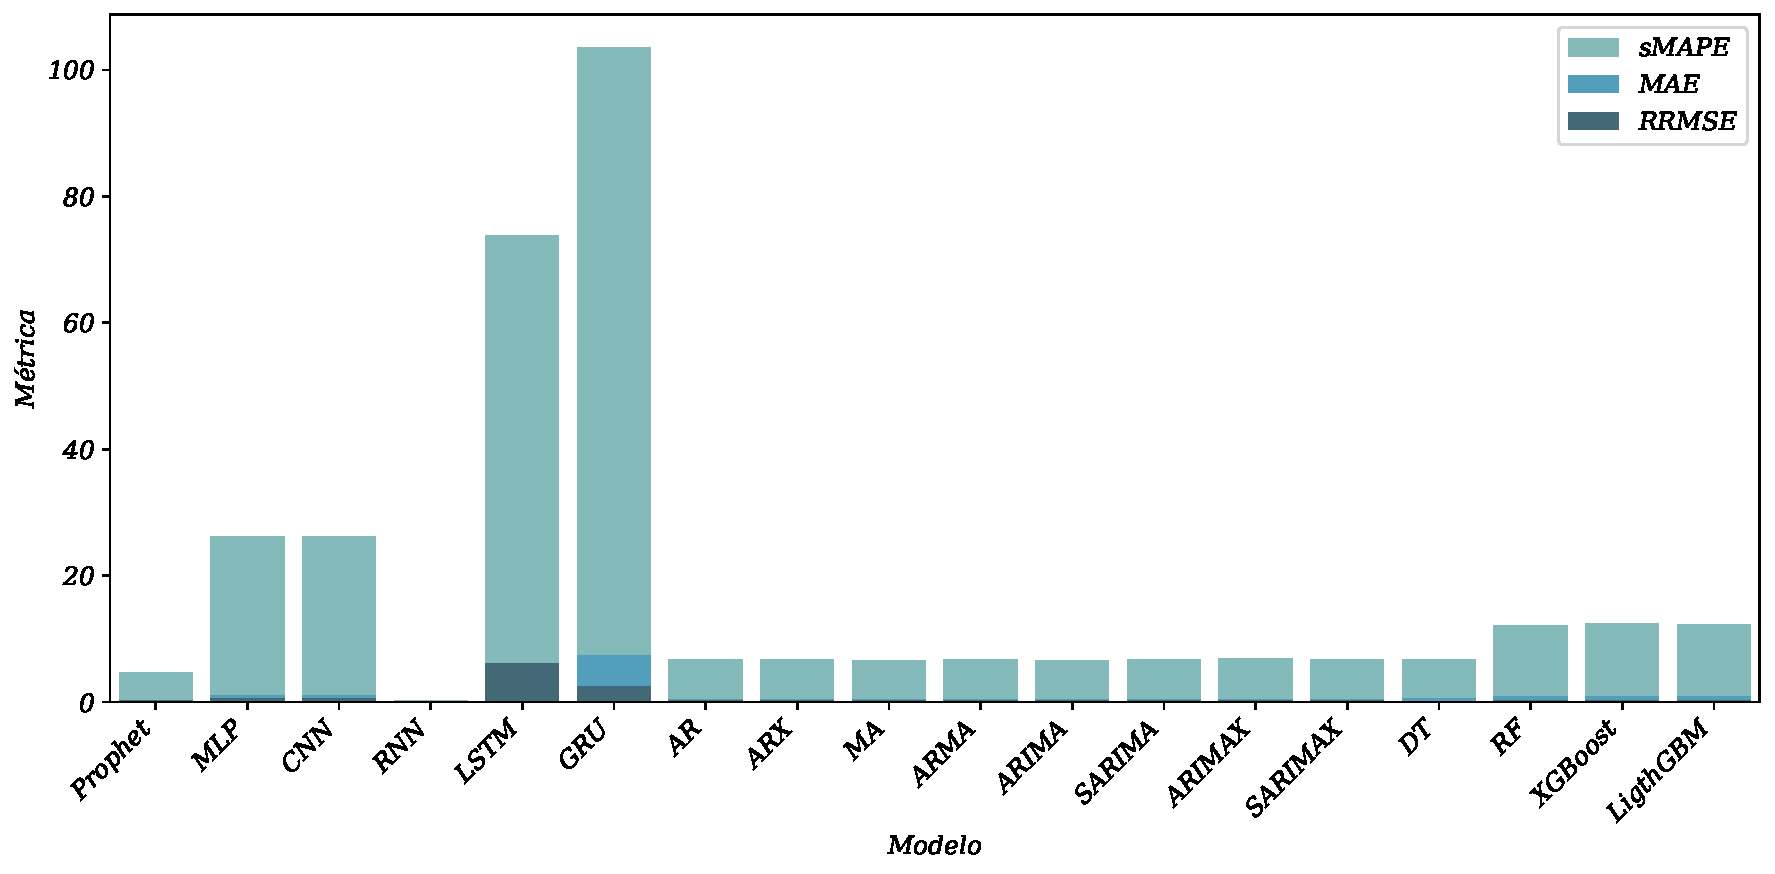
\includegraphics[width=\linewidth]{Resultados/Figuras/metricas_comparacao_modelos}
\end{figure}



A avaliação da eficácia dos modelos ARIMA em previsões de longo prazo emprega o teste de Ljung-Box, conforme detalhado nas Tabelas \ref{tb:lbtrn} a \ref{tb:lbcm} ilustram a acurácia dos modelos ARIMA ao longo do tempo, com valores menores sendo destacados em \textbf{negrito}. Modelos como ARX, ARIMAX e SARIMAX, que incorporam variáveis exógenas, demonstram um desempenho superior nesse contexto. Esses modelos não lineares apresentam uma capacidade de previsão robusta em horizontes temporais mais longos, diferenciando-se positivamente dos outros modelos ARIMA. Na Figura \ref{fig:modelos-arima}, são selecionados os modelos ARIMA e seus antecessores. Esses modelos têm suas limitações, tanto para horizontes de previsão de curto prazo quanto para horizontes de longo prazo. Nessa comparação no gráfico de violino, são combinados vários outros gráficos em um só, como o gráfico de barras e o \textit{boxplot}. Esse gráfico pode fornecer várias informações, mas o objetivo aqui é identificar apenas o melhor modelo entre os modelos ARIMA.

Como essa série não apresentou uma estacionariedade bem definida e os dados não a tornaram estacionária, os modelos que não têm sazonalidade mostraram-se superiores, tais como AR, MA, ARX, ARMA, ARIMA e ARIMAX. O modelo ARIMAX demonstrou ser bastante robusto para este caso, mas mesmo assim, modelos mais básicos como AR e MA ainda apresentaram resultados melhores.

\begin{table}[H]
	\centering		
	\caption{Comparação dos modelos com o teste Ljung Box modelos ARIMA com defasagem de 10 para previsão de longo prazo na demanda d'água.}
	
	\begin{subtable}{0.49\linewidth}
		\centering
		\caption{\textbf{Treinamento}} \label{tb:lbtrn}
		\begin{tabular}{@{}lll@{}}
			\toprule
			Ljung  & Estatística  & Valor \\
			Box & de Teste& de p\\\midrule
			ARX & 59,677 & 0 \\
			AR & 52,312 & 0,265 \\
			MA & 57,268 & 0 \\
			ARMA & 6,945 & 0,731 \\
			ARIMA & \textbf{16,724} & \textbf{0,081} \\
			SARIMA & 48,505 & 0 \\
			ARIMAX & 89,931 & 0 \\
			SARIMAX & 29,093 & 0 \\ \bottomrule
		\end{tabular}
	\end{subtable}
	\hfill
	\begin{subtable}{0.49\linewidth}
		\centering
		\caption{\textbf{Teste}} \label{tb:lbtst}
		\begin{tabular}{@{}lll@{}}
			\toprule
			Ljung  & Estatística  & Valor \\
			Box & de Teste& de p\\\midrule
			ARX & 47,177 & 0 \\
			AR & 49,965 & 0,444 \\
			MA & 77,884 & 0 \\
			ARMA & 1,545 & 0,999 \\
			ARIMA & 5,354 & 0,866 \\
			SARIMA & \textbf{24,663} & \textbf{0,006} \\
			ARIMAX & 36,738 & 0 \\
			SARIMAX & 21,236 & 0,020 \\ \bottomrule
		\end{tabular}
	\end{subtable}
	
	\vspace{0.5cm}
	
	\begin{subtable}{0.49\linewidth}
		\centering
		\caption{\textbf{Validação}} \label{tb:lbvld}
		\begin{tabular}{@{}lll@{}}
			\toprule
			Ljung  & Estatística  & Valor \\
			Box & de Teste& de p\\\midrule
			ARX & 5,108 & 0,884 \\
			AR & 4,360 & 0,930 \\
			MA & 46,252 & 0 \\
			ARMA & 7,515 & 0,676 \\
			ARIMA & 7,738 & 0,654 \\
			SARIMA & \textbf{28,998} & \textbf{0,001} \\
			ARIMAX & 6,115 & 0 \\
			SARIMAX & 4,443 & 0,925 \\ \bottomrule
		\end{tabular}
	\end{subtable}
	\hfill
	\begin{subtable}{0.49\linewidth}
		\centering
		\caption{\textbf{Inteiro}} \label{tb:lbcm}
		\begin{tabular}{@{}lll@{}}
			\toprule
			Ljung  & Estatística  & Valor \\
			Box & de Teste& de p\\\midrule
			ARX &48,870 & 0 \\
			AR & \textbf{49,432} & \textbf{0,035} \\
			MA & 57,629 & 0 \\
			ARMA & 10,053 & 0,436 \\
			ARIMA & 10,053 & 0,436 \\
			SARIMA & 10,053 & 0,436 \\
			ARIMAX & 70,458 & 0 \\
			SARIMAX & 2,897 & 0 \\ \bottomrule
		\end{tabular}
	\end{subtable}
	
	
	\vspace{0.5cm}
	
\end{table}





